\documentclass{article}
\usepackage[backend=bibtex]{biblatex}
\usepackage[utf8]{inputenc}
\usepackage[german]{babel}
\usepackage{caption}
\usepackage[skip=0.5ex]{subcaption}
\usepackage[left=3cm,right=3cm,top=2cm,bottom=2cm]{geometry}

\usepackage{color}
\usepackage{xcolor}
\usepackage{listings}
% define a couple of colors
\definecolor{linkcolor}{rgb}{0.01, 0, 0.38}
\definecolor{commentgreen}{rgb}{0.15,0.42,0.2}
\definecolor{codegray}{rgb}{0.5,0.5,0.5}
\definecolor{stringred}{rgb}{0.6,0.12,0.12}
\definecolor{functionblue}{rgb}{0,0,1}
\definecolor{backcolor}{rgb}{0.95,0.95,0.92}

\usepackage{hyperref}
\hypersetup{
    pdfborder={0 0 0},
    colorlinks=true,
    linkcolor=linkcolor,
    filecolor=linkcolor,      
    urlcolor=linkcolor,
}
\usepackage{bookmark}
\usepackage{booktabs}
\usepackage{textcomp}
\usepackage{array}
\usepackage{graphicx}
\usepackage{parskip} % do not indent first lines

\lstset{language=C++,
  commentstyle=\color{commentgreen},
  keywordstyle=\color{functionblue},
  numberstyle=\tiny\color{codegray},
  stringstyle=\color{stringred},
  basicstyle=\ttfamily\footnotesize,
  breakatwhitespace=false,         
  breaklines=true,                 
  captionpos=b,                    
  keepspaces=true,                 
  numbers=left,                    
  numbersep=5pt,                  
  showspaces=false,                
  showstringspaces=false,
  showtabs=false,                  
  tabsize=2
}

\usepackage{cancel}
\usepackage{mathtools}

\newcommand{\quotes}[1]{''#1''}

\graphicspath{ {./images/} }

\begin{document}
\title{Verteilte Systeme (Burchard 2021) Zusammenfassung}
\author{Jonas Weßner}
\maketitle
\tableofcontents
\newpage				% Neue Seite nach TOC

\section{Overview}

\subsection{Was ist ein Verteiltes System?}
\begin{itemize}
      \item Vile Dinge könnten unter diese Definition fallen, wie z.B. Mulicore Rechner, Cload Rechner oder ein Heimnetzwerk
      \item In der Lehrveranstaltung wird folgende Definition verwendet:\\
            \quotes{Ein verteiltes System ist eine Ansammlung \textit{unabhängiger Computer}, die den Benutzern wie ein \textit{einzelnes kohärentes} System erscheinen.}
      \item Wie betrachten also keine einzelnen großen Parallelrechner und die Verteilung muss dem Nutzer gegenüber verborgen sein (Transparenz)
\end{itemize}

\subsection{Ziele von verteilten Systemen}
\begin{enumerate}
      \item \textbf{Verteilungstransparenz}:\\
            Die Verteiltheit ist dem Nutzer gegenüber verborgen. Der Nutzer weiß nicht, ob und wie das System verteilt ist. Speziell wird folgendes verborgen:
            \begin{enumerate}
                  \item Zugriff:\\
                        Der Zugriff auf alle Ressourcen erfolgt auf gleichem Weg.
                  \item Ort:\\
                        Man kennt den Ort einer Resource nicht.
                  \item Relokation:\\
                        Resourcen können unbemerkt \textit{während der Nutzung} verschoben werden (z.B. wenn sich der Kommunikationspartner einer Mobilfunkverbindung bewegt)
                  \item Migration:\\
                        Resourcen können unbemerkt \textit{zwischen zwei Zugriffen} den Standort wechseln (Bei Abruf 1 antwortet Server x, bei Abruf 2 antwortet Server y)
                  \item Nebenläufigkeit:\\
                        Trotz eines Mehrnutzerbetriebs einsteht der Eindruck eines Einzelnutzerbetriebs.
                  \item Fehler:\\
                        Der Ausfall einer Komponente wird durch das Ersetzen durch eine andere Komponente verborgen.
            \end{enumerate}
      \item \textbf{Offenheit:}\\
            Das System darf aus heterogenen Komponenten mit unterschiedlichen Technologien (z.B Unterschiedlichen OS, HW, Netzwerkprotokollen) bestehen.
      \item \textbf{Skalierbarkeit:}\\
            Das System soll einfach in seiner Größe erweiterbar sein, um die Power der vorhandenen Komponenten bei steigenden Anforderungen mit neuen Komponenten zu verstärken. Z.B. soll es mehrere Datenbankserver oder Webserver geben können.
            Hierbei soll Portierbarkeit und Erweiterbarkeit gewährleistet werden. Anforderungen könnten sein:
            \begin{itemize}
                  \item zusätzliche Rechenpower
                  \item zusätzliche Nutzer
                  \item zusätzlicher Speicherplatz
            \end{itemize}
      \item \textbf{Zuverlässigkeit:}\\
            Das System soll immer zur Verfügung stehen und möglichst Ausfallsicher sein.
\end{enumerate}

\subsection{CAP Theorem (Brewers Theorem)}
\label{sec:CAP_Theorem}
Dieses Theorem betrachtet die 3 Qualitätseigenschaften/Ziele von verteilten Systemen:
\begin{enumerate}
      \item Konsistenz der Daten
      \item Partitionstoleranz:\\
            ein durch einen Netzwerkfehler in Teilsysteme gespaltenes System kann trotzdem weiter arbeiten
      \item Verfügbarket
\end{enumerate}
Das Theorem sagt aus, dass man nur 2 von diesen 3 Zielen erreichen kann, da sie miteinander in Konflikt stehen.
\\
\\
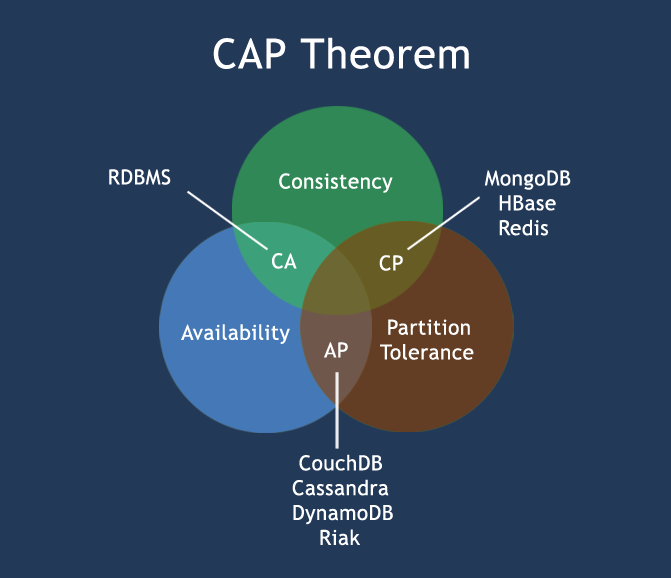
\includegraphics[width=9cm]{CAPTheorem.png}

\subsection{Architekturen für VS}
Ein verteiltes System kann mehreren der folgenden Architekturformen entsprechen. Ein System kann auch heterogen sein und in verschiedenen Teilen verschiedene Architekturen umsetzen.

\subsubsection{Geschichtet (Client-Server)}
Bei einem geschichteten verteilten System werden verschiedene Zuständigkeiten auf mehrere Rechner verteilt. Man unterscheidet zwischen 1-1 Architekturen und Multitier bzw. Multiserver Architekturen.\\
Bei einer \textbf{1-1 Beziehung} wird die Anwendung in genau 2 Teile aufgeteilt. Es handlet sich also, um die klassische Client-Server Architektur. die Anwendung kann hier an beliebigen Teilen unterteilt sein. z.B. kann auf dem Server nur die DB sein, oder auch ein Teil der Anwendung, oder auch noch ein Teil der Benutzerschnittstelle.\\
Eine \textbf{Multitier} Architektur umfasst mehrere Server, die mit einem Client interagieren. Die verschiedenen Schichten, die bei der Informationenverarbeitung durchlaufen werden nennt man auch \textit{layers} oder \textit{tiers}. Es kann z.B. ein \textit{Presentation Layer} geben, dass Daten für den Client darstellt (also wahrscheinlich auf dem Client implementiert z.B. java-script), ein \textit{Service Layer}, das eine API für das Presentation Layer bereitstellt, und ein \textit{Data Access Layer}, das sich um die Daten kümmert (also ein DB Server).

\subsubsection{Objektbasiert}
Objektbasierte Architekturen unterteilen das System in Objekte mit klar definierten Schnittstellen. Ein Objekt kann dann durch Methodenaufrufe auf ein anderes zugreifen. Die Objekte werden dann auf verschiedene Rechner verteilt.\\
Im Gegensatz zur geschichteten Architektur müssen hier also die Schnittstellen noch klarer definiert sein. Die Definitionen überlappen sich aber auch etwas.

\subsubsection{Ereignisbasiert}
Ereignisbasiete Architekturen haben einen Ereignisbus, d.h. ein Kommunikationsmedium, über das Daten asynchron übertragen werden. Wenn ein bestimmtes Ereignis eintrifft, also bestimmte Daten ankommen, kann eine Komponente aktiv werden und die Daten verarbeiten.

\subsubsection{Datenzentriert}
Datenzentrierte Architekturen haben einen gemeinsamen Datenraum (z.B. eine gemeinsame DB), in der Sie sowohl ihre Anfragen als auch Antworten ablegen und so kommunizieren können.
\section{Netzwerkkommunikation}
%________________________________________
\subsection{Kommunikationsarten und Protokolle}
\subsubsection{Verbindungslos \& Verbindungsorientiert}
\textbf{Verbindungsorientierte Kommunikation} zeichnet sich durch die folgenden Eigenschaften aus:
\begin{itemize}
    \item Die Verbindung zwischen Sender und Empfänger wir explizit durch einen Handshake aufgebaut.
    \item Die Übertragung von Paketen wird vom Empfänger bestätigt.
    \item Die Daten werden in der übergeordneten Schicht als verlustfreier geordneter Datenstrom wahrgenommen. Eine gesicherte Verbindung stellt nämlich sicher, dass Pakete ggf. erneut gesendet werden und in Ihrer Reihenfolge beim Empfänger sortiert werden.
    \item Broadcast und Multicast werden nicht unterstützt.
\end{itemize}
\textbf{Verbindungslose Kommunikation} zeichnet sich durch die folgenden Eigenschaften aus:
\begin{itemize}
    \item Es gibt keinen Verbindungsaufbau.
    \item Nachrichten werden ohne warten auf Antwort durch das Netzwerk gesendet.
    \item Die Reihenfolge der Pakete ist nicht garantiert.
    \item Es kann zu Paketverlusten kommen.
    \item Der Anwender muss die Reihenfolge und ggf. das erneute Senden von Nachrichten selbst managen.
\end{itemize}

\subsubsection{Synchrone und Asynchrone Kommunikation}
Je nach Szenario können synchrone oder asynchrone Kommunikation sinnvoll sein.\\
\textbf{Synchrone Kommunikation} zeichnet sich dadurch aus, dass das Senden und Empfangen von Nachrichten den Programmablauf blockiert. Möchte ein Sender also eine Nachricht senden, so würde er warten, bis das Senden möglich ist. Soll eine Nachricht empfangen werden, so wird so lange gewartet, bis die Nachricht eintrifft. Hier macht es Sinn mit Timeouts zu arbeiten.\\
\textbf{Asynchrone Kommunikation} zeichnet sich dadurch aus, dass das Senden oder Empfangen von Nachrichten nicht blockiert. Ein Sender würde also eine Nachricht versenden, egal, ob ein Empfänger bereit ist. Der Empfänger wartet nicht auf eine bestimmte Nachricht, sondern lässt sie puffern und liest sie dann, wenn er dafür bereit ist. Eventuell wird eine callback function aufgerufen, wenn das Event "Nachricht eingetroffen" eintrifft (z.B. über POSIX Signale).

\subsubsection{Qualitätsparameter von Netzwerken}
\begin{itemize}
    \item \textbf{Latenz:}\\
          Die minimale Verzögerung zwischen Sender und Empfänger. Also die Zeit, die benötigt wird, wenn man eine leere Nachricht versenden würde.
    \item \textbf{Datentransferrate:}\\
          Datenmenge, die innerhalb eines bestimmten Zeitraums maximal zwischen den Prozessen übertragen werden kann.
    \item \textbf{Nachrichtentransferzeit:}\\
          Die tatsächliche Verzögerung beim Versenden einer Nachricht. Sie setzt sich zusammen aus der Latenz und der Zeit, die für die pure Übertragung der Nachricht gebraucht wird:\\
          Latenz + Nachrichtenlänge / Datentransferrate
    \item \textbf{Durchsatz:}\\
          Menge der Bits, die pro Zeiteinheit über eine Verbindung übertragen werden.
    \item \textbf{Bandbreite:}\\
          Maximal möglicher Durchsatz des Netzwerks.
\end{itemize}

\subsubsection{Protokolle \& Internet}
Im Internet werden Daten übertragen, indem Sie mehrere logische Schichten und damit verbundene Protokoll durchlaufen (siehe OSI-\& TCP/IP-Modell).\\
Die Nachricht wird zunächst von der Anwendungsschicht aus mit puren Nutzdaten formuliert. Um diese Daten zu übertragen werden Protokolle benutzt, die sich dadurch auszeichnen, dass sie die Nachricht um Meta-Informationen erweitern und Regeln definieren, wie mit der Nachricht und den Protokollinformationen umgegangen werden soll. Ein paar Protokolle wollen wir hier noch kurz genauer betrachten:\\
\\
\textbf{IP - Internet Protokoll}\\
Das Internet Protocol ist die Implementierung der \textit{Internetschicht} (TCP/IP) bzw. \textit{Vermittlungsschicht} (OSI). Das IP bildet die Grundlage für alle relevanten Protokolle, die über das Internet Daten versenden möchten.\\
Das IP abstrahiert die verschiedenen möglichen Übertragungswege und Teilnetze, die im Internet existieren zu einem gemeinsamen Adressraum, der durch IP-Adressen definiert wird. Mittels dieser Form von Adressierung und Routing (der Wegfindung) kann mithilfe des IP eine Nachricht von einem Sender zu einem Empfänger gelangen.\\
Der Header des IP enthält vor Allem die Source- und Destination-IP-Address und eine TTL (Time to Live).\\
Das IP ist ein Verbindungsloses Protokoll, auf dessen Basis dann verbindungsorientierte Protokolle wie TCP arbeiten können.\\
\\
\textbf{UDP - User Datagram Protocol}\\
Das UDP ist eine Implementierung der Transportschicht (TCP/IP).\\
Das UDP verwendet Ports, um eine Nachricht dem richtigen Prozess auf dem Zielrechner zukommen zu lassen. Es erweitert also das IP von einer Rechner-Rechner Verbindung zu einer Prozess-Prozess verbindung. Außerdem können auch Checksums mitgesendet werden, um fehlerhaft Pakete beim Empfänger zu erkennen und zu verwerfen.\\
UPD ist eine sehr leichtgewichtiges verbindungsloses Protokoll, das benutzt wird, wenn Daten zeitkritisch ankommen müssen, aber Paketverluste nicht tragisch sind (z.B. Telefonie, Live-Streaming...).
Bei UDP entsteht wesentlich weniger Overhead als bei TCP, da keine Bestätigungen für Pakete gesendet werden.
UDP ist außerdem Broadcast und Multicast fähig. UDP ist grundsätzlich ein unidirektionales Protokoll, es kann jedoch in beide Richtungen gleichzeitig verwendet werden, um eine beidseitige Kommunikation zu erreichen.\\
\\
\textbf{TCP - Transmission Control Protocol}\\
Das TCP ist eine Implementierung der Transportschicht (TCP/IP).\\
TCP ist ein verbindungsorientiertes Protokoll. TCP benutzt auch, wie UDP, Ports als Adresszusatz. Die Kommunikation über TCP ist bidirektional. Multicasts oder Broadcasts sind mit TCP \textbf{nicht} auf einfache Weise möglich.\\
Beim TCP wird der Verbindungsaufbau durch einen 3 Wege Handshake eingeleitet. Danach werden Pakete versendet. Jedes Paket muss vom Empfänger bestätigt werden, jedoch können mehrere Pakete gleichzeitig bestätigt werden. Nicht bestätigte Pakete werden vom Sender nach gewisser Zeit erneut versendet. Der Verbindungsabbau wird wird ebenfalls mit einem 3-Wege-Handshake durchgeführt.\\
Der Header des TCP enthält im Wesentlichen die Ports beider Kommunikationspartner, eine Sequence-Number, welche die Reihenfolge der Pakete festlegt, eine Acknowledgement-Number, welche angibt welches TCP Paket als nächstes erwartet wird und eine Reihe von Options, die weitere kleinere Informationen übermitteln.\\
\\
\textbf{HTTP - Hypertext Transfer Protocol}\\
Das HTTP baut auf TCP auf. Bei TCP ist die Reihenfolge und das ankommen der Daten garantiert. Jedoch segmentiert TCP selbstständig die Daten als Pakete. Der Empfänger kann also zu keinem Zeitpunkt sicher sein, ob die Nachricht schon komplett eingetroffen ist, oder ob noch weitere TCP Pakete folgen. HTTP fügt TCP nun noch Header-Informationen hinzu, die unter anderem Anzeigen wie lang die Nachricht ist. Dadurch kann der Empfänger feststellen wann eine Nachricht endet und eine weitere Beginnt.

%________________________________________
\subsection{Sockets}
Sockets sind bidirektionale Kommunikationsendpunkte, die im Speicher als Objekt repräsentiert werden und vom Betriebssystem bereitgestellt werden. Sockets werden in fast allen Programmiersprachen unterstützt (C, C++, C\#, PHP...). Mittels Sockets kann ein Prozess mit einem anderen Kommunizieren. Mittels TCP- und UDP-Sockets kann die Kommunikation über Netzwerke erfolgen. D.h. der Kommunikationsmechanismus wird vom OS so bereitgestellt, dass ein Rechner mit einem Systemaufruf eine Nachricht an einen anderen Rechner senden kann, der diese mit einem Systemaufruf annehmen kann:\\

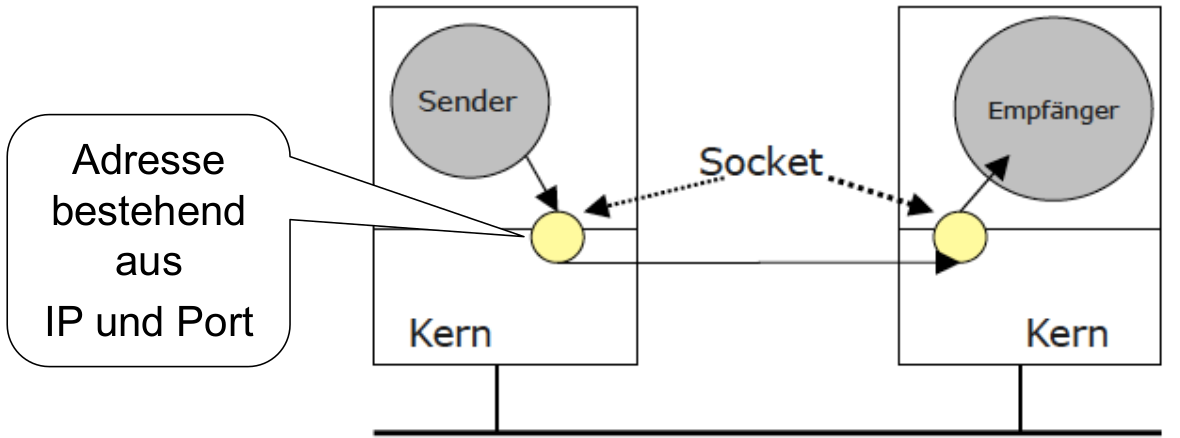
\includegraphics[width=10cm]{Sockets.png}

\subsubsection{UPD Sockets}
Das UDP ist zwar ein unidirektionales Protokoll, doch ein Socket-pair kann trotzdem bidirektional verwendet werden. Beide Empfänger benutzen dann jeweils UDP für eine Datenübertragung in eine Richtung aber über das gleiche Socket.\\
Bei der Benutzung von UDP Sockets wird durch einen Aufruf von \textit{send} genau ein Paket gesendet. Ist die Datenmenge zu groß, dann muss der Sender die Nachricht händisch in mehrere Pakete unterteilen.
Bei der Programmierung von UDP Sockets ist der Entwickler für folgendes verantwortlich:
\begin{enumerate}
    \item Senden jedes einzelnen Pakets (1 Paket bis 64kB)
    \item Korrektur der Reihenfolge der Pakete beim Empfänger
    \item Fehlerkorrektur
    \item Segmentierung großer Datenvolumen
\end{enumerate}
Für UDP stehen unter anderem folgende POSIX-Systemaufrufe zur Verfügung:
\begin{itemize}
    \item \textbf{socket} - Socket erzeugen
    \item \textbf{bind} - Socket an eine IP-Adresse binden
    \item \textbf{sendto}
    \item \textbf{recvfrom}
    \item \textbf{close}
    \item \textbf{setsockopt} - optionale Optionen (Puffergröße, REUSE\_ADDR, ...)
\end{itemize}

\newpage
\textbf{Hier ein Beispiel für die Programmierung mit UDP-Sockets:}\\

\textit{Code des Servers (Empfängers):}
\begin{lstinputlisting}[language=C++]
    {../src/UDP_receive/main.cpp}
\end{lstinputlisting}
\newpage
\textit{Code des Clients (Senders):}
\begin{lstinputlisting}[language=C++]
    {../src/UDP_send/main.cpp}
\end{lstinputlisting}


\subsubsection{TCP Sockets}
Die Benutzung von TCP erfordert im Gegensatz zur Benutzung von UDP zu Beginn der Kommunikation einen Verbindungsaufbau.\\
Der Server muss dafür seine IP Adresse und seinen Port  mit \textit{bind} an den Socket binden. Dann muss er mit \textit{listen} den Socket als passiven Socket markieren. Das bedeutet, dass er in der Zukunft über diesen Socket auf Anfragen warten möchte. Nun muss der Server \textit{accept} aufrufen. Accept blockiert so lange, bis eine Connection Request eines Clients eintrifft und gibt dann einen neuen Socket zurück, der mit dem Socket des Clients verbunden ist und zur Kommunikation genutzt werden kann. Der ursprüngliche Socket kann dann benutzt werden, um weitere Anfragen anzunehmen. Mit den Aufrufen \textit{send} und \textit{recv} können Sender und Empfänger bidirektional Daten versenden.\\
Ein wesentlicher Unterschied zwischen TCP und UDP ist, dass bei TCP eine beliebig große Menge an Daten mit einem Aufruf von send übertragen werden können. Der TCP Protokollstack kümmert sich dann um die Segmentierung der Daten. Das bedeutet, dass wir hier einen Datenstrom und nicht ein einzelnes Datenpaket übertragen. Für den Empfänger (Client) bedeutete das, dass er nicht wissen kann wie viele Pakete eintreffen und wann die Nachricht komplett übertragen wurde. Ein Aufruf von \textit{recv} gibt dann nicht wie bei UPD-sockets die Daten genau eines Aufrufes von \textit{send} zurück, sondern die Daten aller Pakete, die bisher eingetroffen sind. Diese Pakete können nur ein Teil einer Nachricht sein oder auch von mehreren separaten Nachrichten stammen. Daher benötigt man für eine sichere Anwendung mit TCP auch noch ein Format (z.B. HTTP), das spezifiziert wann eine Nachricht zu Ende ist und eine weitere Nachricht beginnt.\\
\\
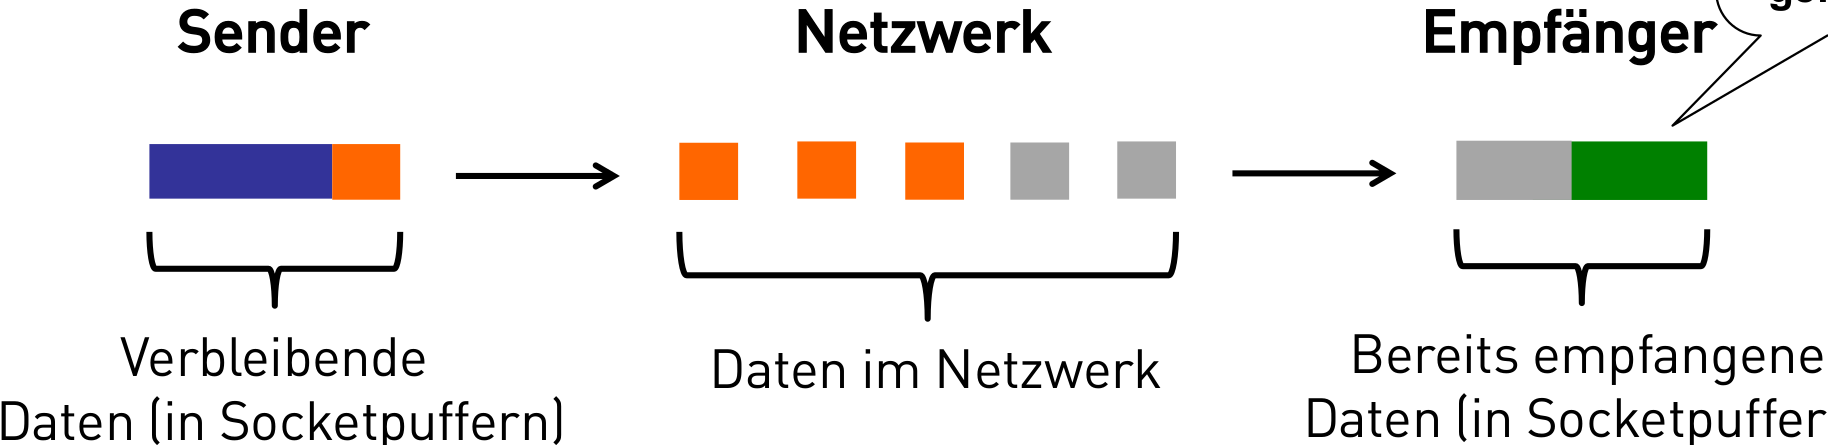
\includegraphics[width=11cm]{images/TCP_packets.png}
\\
\\
Für TCP Sockets stehen unter anderem folgende POSIX-Systemaufrufe zur Verfügung:
\begin{itemize}
    \item \textbf{socket} - Socket erzeugen
    \item \textbf{bind} - Socket an IP Adresse und Port binden
    \item \textbf{send}
    \item \textbf{recv}
    \item \textbf{connect} - wird vom client aufgerufen, um eine Verbindung zu initiieren
    \item \textbf{listen} - wird vom Server aufgerufen, um sein Socket als passives, also lauschendes Socket zu kennzeichnen
    \item \textbf{accept} - wird vom Server aufgerufen, um auf eine Verbindungsanfrage eines Clients zu warten
    \item \textbf{close}
\end{itemize}

\newpage
\textbf{Hier ein Beispiel für die Programmierung mit TCP-Sockets:}\\

\textit{Code des Servers:}
\begin{lstinputlisting}[language=C++]
    {../src/TCP_server/main.cpp}
\end{lstinputlisting}
\newpage
\textit{Code des Clients:}
\begin{lstinputlisting}[language=C++]
    {../src/TCP_client/main.cpp}
\end{lstinputlisting}

\subsubsection{Parallelisierung und \textit{select}}
Socketfunktionen \textit{connect}, \textit{accept}, \textit{send}, \textit{recv} arbeiten by default synchron und blockieren bis die Operation durchgeführt werden kann. Man bräuchte also n Threads, um eine Menge von n Sockets gleichzeitig zu Managen, obwohl die einzelnen Threads die meiste Zeit bloß blockiert sind und auf Aktivität warten. Es gibt mehrere Möglichkeiten dieses Problem zu beheben:\\
\textbf{Non Blocking Sockets}\\
Man kann Sockets aber auch beim Erzeugen in den Modus \textit{NONBLOCK} setzen, indem man die Funktion \textit{fcntl} mit dem Argument \textit{O\_NONBLOCK} für den Socket aufruft. Dann kehrt der Systemaufruf sofort zurück und der Rückgabewert gibt an, ob der Aufruf erfolgreich war.
So kann man also über eine Liste von Sockets iterireren und feststellen, ob einer der Sockets bereit für eine Aktion ist. So kann ein Prozess/Thread mehrere Sockets überwachen anstatt bei einem Socket dauerhaft blockert zu sein.\\
\textbf{Select}\\
Die Funktion \textit{select} setzt das gleiche Prinzip um. Ihr kann eine Liste von Sockets übergeben werden, die sie überwacht. Die Funktion blockiert bis einer der Sockets für die gewünschte Operation bereit ist. Dann kann man den gewünschten Socket finden und ihn bearbeiten. Bei der Nutzung von \textit{select} kann auch noch ein Optionaler Timeout angegeben werden.\\
Der Ablauf beim Benutzen von \textit{select} ist dann wie folgt:\\
\begin{enumerate}
    \item Alle Sockets mittels \textit{FD\_SET} in die eine Datenstruktur vom Typ \textit{fd\_set}(file descriptor set) eintragen.
    \item Die Funktion \textit{select} mit den Parametern aufrufen, die angeben auf welche Aktion man wartet.
    \item Nachdem select zurückgekehrt ist mittels \textit{FD\_ISSET} prüfen welcher Socket bereit ist.
    \item Diesen Socket bearbeiten (evtl. einen neuen Thread dafür erzeugen)
    \item Wieder bei 1. anfangen, um die Sockets neu in die Liste einzutragen, da \textit{select} destruktiv ist.
\end{enumerate}

\textbf{Hier ein kleines unvollständiges Beispiel:}\\

\begin{lstinputlisting}[language=C++]
    {../src/select_example.cpp}
\end{lstinputlisting}
\newpage

%________________________________________
\subsection{Remote Procedure Calls (RPC)}

Remote Procedure Calls sollen die Kommunikation über Sockets abstrahieren, die Komplexität verbergen und eine einfachere Schnittstelle für den Datentransfer über Netzwerke bereitstellen.
\subsubsection{Funktionsweise}
Es gibt eine Funktionssignatur (oder mehrere), also eine Schnittstelle, die auf Server- und Client-Seite gleich sein muss. Die Implementierung dieser Funktion befindet sich auf dem Server. Wenn der Client die Funktion aufruft soll nun der Server den Programmcode ausführen und den Rückgabewert zum Client zurückgeben. Für den Client soll es so aussehen, als hätte er eine lokale Funktion aufgerufen. Das läuft dann so ab:
\begin{enumerate}
    \item Der Client ruft die Funktion auf
    \item Das RPC Framework ruft eine sogenannte Stub-Funktion auf, die die Anfrage auf den Funktionsaufruf, sowie die Funktionsparameter serialisiert (Marshalling) und diese Daten über das Netzwerk via Sockets an den Server sendet
    \item Die Stub-Funktion auf dem Server wird übernimmt das Empfangen der Daten über den Socket und deserialisiert die Daten
    \item Die Implementierung der vom Client aufgerufenen Funktion wird mit den über das Netzwerk übermittelten Parametern ausgeführt.
    \item Eine Stub-Funktion des Servers serialisiert den Rückgabewert und sendet ihn über den internen Socket an den Client
    \item Die Funktion des Clients kehrt zurück, so als ob sie lokal (aber merkbar langsamer) ausgeführt worden wäre
\end{enumerate}

Die Implementierung der Stub-Funktionen, die die Abstrahierung der Datenübertragung schaffen, kommen von einem RPC-Framework. Es gibt viele RPC-Frameworks, alle implementieren das oben genannte Geschehen in ihrer eigenen Weise. Damit das Framework weiß an welchen Server der RPC gesendet werden soll, muss im Rahmen der Initialisierung auch noch die IP-Adresse und der Port des Servers angegeben werden. Bei der Initialisierung können je nach Framework auch noch zusätzliche Informationen angegeben werden, wie z.B.
\begin{itemize}
    \item Timeout bis das Warten auf den Rückgabewert des Servers abgebrochen wird
    \item Netzwerkprotokoll: UDP oder TCP, eventuell auch darauf aufbauend HTTP
    \item Datenformat: Binär, JSON, XML...
\end{itemize}

\subsubsection{Vorteile von RCP gegenüber Sockets}
\begin{itemize}
    \item Konkrete Aufrufe von Operationen über Sockets werden abstrahiert und vereinfacht
    \item Implementierung der Datenübertragung über Sockets wird einmalig durch RPC-Framework performant implementiert
    \item Konvertierung unterschiedlicher Zahlendarstellungen z.B. 1er vs. 2er Komplement, Big-Endian vs. Little Endian wird durch das Framework gewährleistet.
\end{itemize}

\subsubsection{Einschränkungen und Nachteile von RPC}
\begin{itemize}
    \item Bei Funktionsaufrufen kann kein call-by-reference und keine Übergabe mittels von Pointern erfolgen, weil der Adressraum des Callers nicht der gleiche Adressraum wie der des Ausführers der Funktion ist.
    \item Datenübertragung über RCP ist standardmäßig unverschlüsselt und kann abgehört werden
    \item Die Abstrahierung vereinfacht zwar die Datenübertragung für den Programmierer, aber man verliert dadurch natürlich auch Kontrolle über die Implementierung und die Analyse von Fehlern kann weniger präzise durchgeführt werden.
    \item RPC macht zwar den Aufruf der Funktionen auf dem Server durch das Verbergen der Sockets einfacher (\textit{Einfacher Zugriff auf Ressourcen}) aber in Bezug auf die anderen Qualitätsmerkmale Verteilter Systeme, \textit{Verteilungstransparenz, Offenheit, Skalierbarkeit, Zuverlässigkeit}, hilft uns RPC noch nicht wirklich weiter.
\end{itemize}

\subsubsection{Generelles Vorgehen bei der Programmierung mit RPCs}
Zunächst einmal stellt sich die Frage, woher der Code für die Stub-Funktionen kommt, die uns die Arbeit mit der Netzwerkübertragung vereinfachen. Dafür wird vom RPC-Framework eine Interface-Definition-Language (IDL) bereitgestellt, die i.d.R. auch für jedes Framework verschieden ist. Mithilfe dieser sehr einfachen Sprache definieren wir das Interface, also die Signaturen, der Funktionen, die über RPC erreichbar sein sollen. Das RPC-Framework stellt auch noch einen für die IDL spezifischen Compiler bereit, der aus der dem IDL-Code dann den \textbf{Source-Code} für die Stubs auf Server- und Clientseite generiert.
Das bedeutet also, dass die IDL gezielt als Cross-Platform Lösung designed ist, sodass der Source-Code der Stubs dann für beliebige Programmiersprachen generiert werden kann. Dieser Source-Code kann dann dann mit dem Source-Code des eigentlichen restlichen Programm zusammen kompiliert werden.\\

Die Generelle Vorgehensweise beim Programmieren mit einem RPC-Framework lässt sich wie folgt beschreiben:
\begin{enumerate}
    \item Die Funktionen der Schnittstelle auf dem Server implementieren
    \item Die Funktion an geeigneten Stellen im Code des Clients verwenden
\end{enumerate}

\textbf{Konkrete Implementierungen von RPC (RPC-Frameworks)}\\
\begin{itemize}
    \item \textbf{Sun ONC-RPC:} Das älteste und \quotes{originale} Framework, das nur die Sprache C unterstützt. Wird in diesem Dokument nicht genauer betrachtet
    \item \textbf{Apache Thrift:} Ein relativ modernes Framework, das viele Sprachen, wie C, C++, Java, PHP, Python u.v.m. unterstützt
    \item \textbf{Protocol Buffers - Protobuf:} Protocol Buffer ist ein Verfahren zur Serialisierung und Deserialisierung von Daten zu und von einem einheitlichen Format, das von Google entwickelt wurde. Das heißt beim Verwenden von Protobuf wird die Kommunikation noch vollständig vom Programmierer gelöst (also vermutlich über Sockets). Es ist also ein Datenformat, wie XML, das aber den Anspruch hat performanter und sparsamer zu sein.
    \item \textbf{gRPC:} ist ein modernes RPC-Framework von Google, das sehr ähnlich zu Apache Thrift ist, welches auf Protobuf basiert
    \item \textbf{XML-RPC:} Legt den Focus auf das Datenübertragungsformat, welches hier mittels XML läuft und dann über HTTP übertragen wird. Damit ist diese RPC Implementierung nicht besonders performant, aber sehr einfach, sodass sie auch leicht selbst mit einem HTTP-fähigen Server implementiert werden kann. Man muss nur aus dem XML ablesen welche Funktion aufgerufen werden soll und den Rückgabewert dann wieder als XML zurücksenden
    \item \textbf{JSON-RPC: } wie XML-RPC nur mit JSON
\end{itemize}

\subsubsection{Programmieren mit Apache Thrift}


Wir gehen schrittweise vor:\\
\\
\textbf{1. Definition des Interfaces in der IDL:}\\
Dazu erstellen wir das file \textit{example.thrift} mit einer einfachen Signatur einer Beispielfunktion, die zwei Zahlen addieren soll. Die Funktion \textit{ping} ist eine Funktion, die Serverseitig keine Implementierung bekommen soll. Sie soll sofort zurückkehren. Anhand ihrer Ausführungszeit kann man also ungefähr die Round-Trip-Time der RPC-Schnittstelle bestimmen.
\begin{lstinputlisting}[]
    {../src/RPC_Thrift/example.thrift}
\end{lstinputlisting}

Dabei wird ein Directory \textit{gen-cpp/} erstellt, das dann die Source Files für den Client, sowie ein Template für eine Implementierung auf Serverseite (Example\_server.skeleton.cpp) enthält. Alle files können im Ordner \textit{src/RPC\_Thrift/} dieses git-Repositories gefunden werden.\\
Das File für den Server können wir in ein anderes Directory kopieren und anpassen, vor allem die Implementierung der Funktion(en) des RPC-Interfaces ist natürlich notwendig. Die anderen generierten Files können wir so belassen, wie sie sind.\\
Wir werden feststellen, dass die generierten Dateien Bibliotheken includieren, die wir zuerst noch auf dem Host System installieren müssen. Dazu müssen wir das git-Repository clonen und die für die Installation erforderlichen Schritte durchführen. Wenn Thrift installiert ist werden die erforderlichen Dateien normalerweise unter \textit{/usr/local/include/thrift} abgelegt. Die Schritte zur Installation finden sich im Root-Verzeichnis dieses Repositories und sind zur Zeit folgende:

\begin{lstinputlisting}[]
    {../src/RPC_Thrift/docs/install-thrift-library.txt}
\end{lstinputlisting}

Das Programm muss dann mit den -lthrift Flag kompiliert werden. In dem Beispiel haben wir Example\_server.skeleton.cpp in das root directory verschoben und zu server-main.cpp umbenannt. Alle Files finden sich auch im \textit{src/RPC\_Thrift/} dieses Repositories. Simples Makefile:

\begin{lstinputlisting}[]
    {../src/RPC_Thrift/Makefile}
\end{lstinputlisting}

\textbf{3. Implementierung des Server-Codes:}\\
Die Implementierung des Servers ist sehr einfach, weil die Konfiguration schon im Code Template vorgegeben ist. Optional können wir hier noch den Port ändern. Wir müssen eigentlich also nur noch die tatsächliche Logik der Funktionen der Schnittstelle ergänzen. Diese Implementierung gestaltet sich bei unseren simplen Beispielfunktion natürlich sehr einfach (return a+b;). Hier nochmal das komplette Serverfile, das in \textit{src/RPC\_Thrift/server-main.cpp} zu finden:

\begin{lstinputlisting}[]
    {../src/RPC_Thrift/server-main.cpp}
\end{lstinputlisting}

\textbf{4. Implementierung des Client-Codes:}\\
Die Implementierung des Clients ist genau so simpel. Nur haben wir hier kein Template, sondern müssen selbst die Konfiguration vornehmen. Die ist aber im Grunde einfach und immer gleich, kann also kopiert werden. Wichtig ist natürlich nur den Server Namen und den Server Port anzupassen.\\
Nach der Konfiguration rufen wir die Funktion auf und schließen den Kanal wieder. Wir sollten uns bewusst sein, dass es sich um einen Funktionsaufruf handelt, der über Sockets kommuniziert wird. Daher müssen wir mit Verzögerungen und eventuell auch Exceptions rechnen. Der Code findet sich auch in \textit{src/RPC\_Thrift/client-main.cpp}:

\begin{lstinputlisting}[]
    {../src/RPC_Thrift/client-main.cpp}
\end{lstinputlisting}

\textbf{5. Starten}\\
Dazu muss der Source-Code, wie in \textit{src/RPC\_Thrift/Makefile} angegeben, kompiliert werden. Dann sollte zuerst der Server und dann der Client gestartet werden.
\section{Middleware}

\subsection{Was ist Middleware}

Eine Middleware ist eine Technologie, die die Kommunikation über ein Netzwerk ermöglicht und auf Sockets basiert. Von einer Middleware werden gewisse Funktionalitäten erwartet, die sie von der bloßen Netzwerkkommunikation unterscheiden:

\begin{itemize}
    \item Es wird eine Infrastruktur mit Lösungen für Standardaufgaben bereitgestellt.
    \item Es wird Verteilungstransparenz z.B. Ortstransparenz ermöglicht.
    \item Es werden ggf. zusätzliche vom Einsatzbereich abhängige Funktionalitäten bereitgestellt.
\end{itemize}


\subsection{Message-oriented Middleware}

Die Message-oriented Middleware (MoM) überträgt - so wie der Name es schon verrät - Daten als einzelne Nachrichten. MoMs bieten die folgenden Features:

\begin{itemize}
    \item Warteschlangen (queues) für die Zwischenspeicherung von Nachrichten
    \item Infrastruktur zur Benennung von Kommunikationsendpunkten, also einen Namensdienst, der Kommunikationspartner anhand von Namen oder IDs anstatt von IP-Adresse und Port identifiziert.
    \item Funktionen zur Akkumulierung von Nachrichten. Einzelne Nachrichten können automatisch akkumuliert werden und nur das Ergebnis übertragen werden.
    \item Direkte Unterstützung von Broadcast ohne spezielle IP-Adressen
\end{itemize}

Der Nachrichtentransfer über MoM ist asynchron und wird auch \textbf{Message Passing} genannt. Die Daten werden beim Senden in eine Warteschlange gegeben und bei Bedarf abgefragt. Auf diese Weise können Nachrichten zu jeder Zeit gesendet und empfangen werden ohne darauf zu warten, dass der Kommunikationspartner bereit ist.\\
Auf diese asynchrone Kommunikation kann man bei Bedarf natürlich eine synchrone Kommunikaiton aufbauen, indem man z.B. ein Request-Reply-Modell implementiert.

Im folgenden wollen wir nun Beispiele für MoM kennenlernen, um besser zu verstehen, wie eine MoM aussehen kann.

\subsubsection{MQTT}

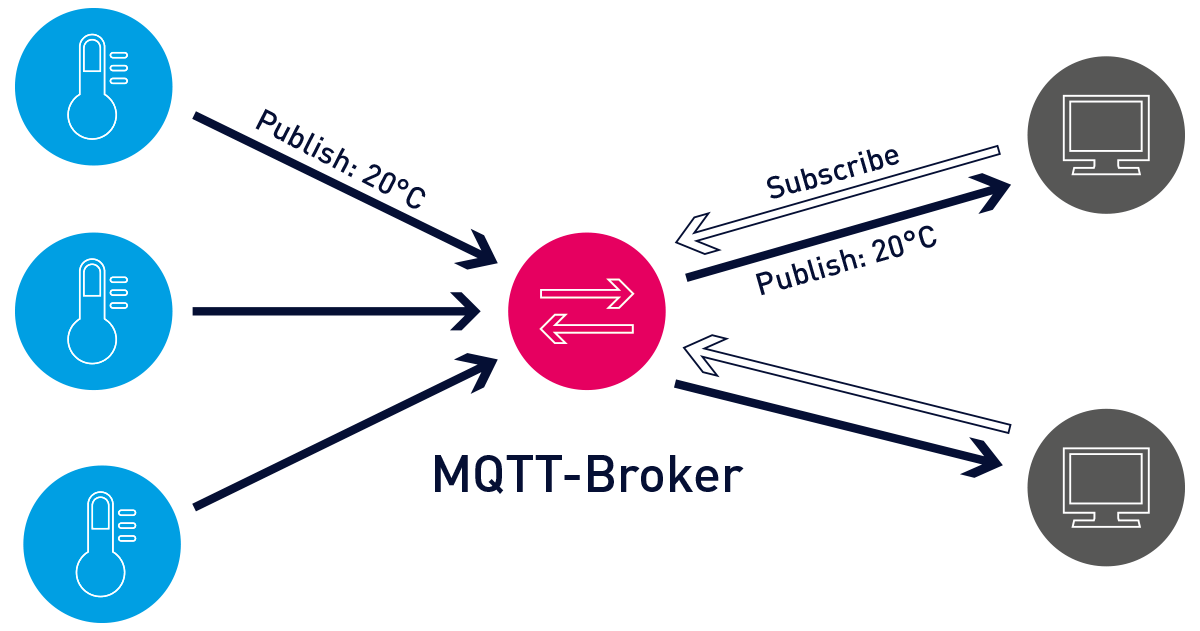
\includegraphics[height=170px]{MQTT.png}

Bei MQTT gibt es einen Broker, der der Nachrichten empfängt und ausliefert. Er enthält eine Warteschlange und optional eine Datenbank in der Nachrichten persistent gespeichert werden können. Die Publisher müssen sich beim MQTT-Broker registrieren und können dann Nachrichten an ihn senden. Die Subscriber können dann diese Nachrichten abfragen. Nachrichten können einem gewissen \textit{Topic} zugeordnet werden. Topics sind eine Einteilung in semantische Gruppen von Nachrichten. So können Subscriber dann nur Nachrichten zu den Topics abfragen, die für sie interessant sind.\\
Die Publisher und Subscriber müssen nur noch die IP-Adresse des Brokers kennen. Der Broker implementiert Logik, um sich zum Zeitpunkt der Registrierung die IP-Adresse des Teilnehmers zu merken. Somit entsteht Ortstransparenz. Nur der Broker kennt nun die genauen Teilnehmer. Die anderen Komponenten des verteilten Systems senden und empfangen jetzt Nachrichten ohne zu Wissen zu wem sie gelangen oder von wem sie kommen. Man kann nun für den Broker eine vorgegebene Implementierung, wie Mosquitto, benutzen. Auf diese Weise muss man sich mit dem Teil, der die Logik der Middleware implementiert, nicht mehr kümmern und kann die vollen Vorteile der MoM ausspielen.\\
MQTT wird vor allem gerne im Zusammenhang mit dem IoT und Sensoren genutzt.

\subsubsection{MPI \& MPICH}

MPI (Message Passing Interface) ist ein Standard, der den Nachrichtenaustausch bei parallelen Berechnungen in verteilten Systemen betrifft. MPI ist folglich im Zusammenhang mit High Performance Computing (HPC) relevant, also dort, wo enorme Rechenlast auf Cluster verteilt werden soll. Dabei sind alle Rechenprozesse meist gleichartig, führen also den selben Code mit unterschiedlichen (Teil-)Daten aus. MPICH ist eine Implementierung dieses Standards.\\
MPICH stellt ein CLI zur Verfügung mit dem mehrere Instanzen eines Programms zur Parallelen Ausführung gestartet werden können. Z.B.:\\
\textbf{\$ mpiexec -n 36 ./myProgram}\\
In dem Programm selbst kann man dann die MPICH Bibliothek benutzen, um die Kommunikation zwischen den Prozessen zu implementieren. Das CLI übergibt den Prozessen als Parameter dann weitere Informationen, die im Programmcode dann durch einen einfachen Aufruf von MPI\_Init genutzt werden, um das MPI des Prozesses zu initialisieren. Dazu gehört auch eine ID. Man kann dann sein Programm so schreiben, dass alle Prozesse eine Berechnung durchführen und ihr Ergebnis an den Prozess mit ID=0 schicken, der dann alle Ergebnisse ausgibt. Für die einfache Akkumulierung von Werten, z.B. Summen- oder Produktbildung, kann direkt beim Senden der Daten ein Funktionsaufruf benutzt werden, der die Akkumulierung durchführt und nur das Ergebnis an den Empfänger überträgt. MPI hat den Anspruch fehlerfreier Nachrichtenübertragung. Falls ein interner Fehler auftritt, wird die Übertragung erneut versucht bis sie erfolgreich ist (retransmission). Das bedeutet, dass der Programmierer sich nicht um Fehlerbehandlung kümmern muss (Fehlertoleranz), aber auch, dass er auch keine Fehlerbehandlung durchführen könnte, wenn es doch zu internen Fehlern kommt (Kontrollverlust). Es folgt ein kurzes Programmierbeispiel:

\begin{lstinputlisting}[language=C++]
    {../src/MPICH/main.cpp}
\end{lstinputlisting}

\subsubsection{Apache Kafka}

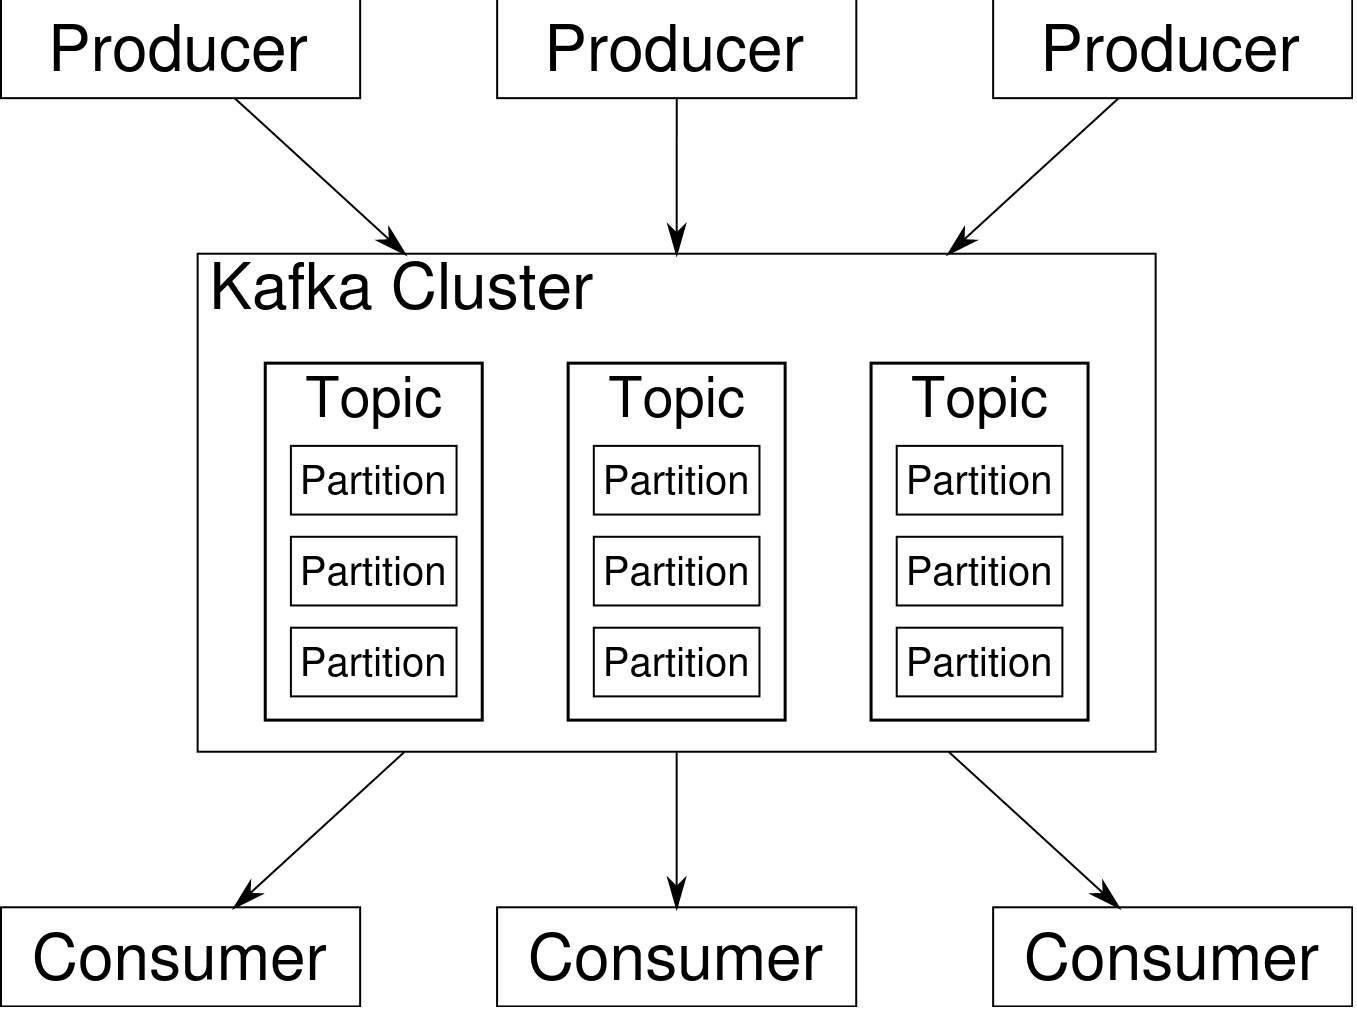
\includegraphics[height=170px]{ApacheKafka.png}

Apache Kafka ist eine Open Source Middleware, die ähnlich wie bei MQTT ein Publish-Subscribe System implementiert. Der wesentliche Unterschied ist, dass Kafka statt Nachrichten Datenströme verarbeitet und auf High-Performance und High-Scalability ausgelegt ist. Ursprünglich von der Firma LinkedIn entwickelt sollte Kafka dazu verwendet werden, Logging Daten von sehr großen Rechnernetzen in Echtzeit zu sammeln. Mit den gesammelten Daten konnten dann Echtzeit-Analysen über das Gesamtsystem erstellt werden.\\
Bei Kafka gibt es, wie bei MQTT, Publisher/Producer, Subscriber/Consumer und Broker. Bei Kafka können die Broker und die Subscriber geclustert werden, um Ausfallsicherheit und hohe Skalierbarkeit zu gewährleisten.

\subsection{Object-oriented Middleware}

Object-oriented Middleware ist eine Gruppe von Middleware, bei der Objekte einer Programmiersprache übertragen werden können. Im folgenden wollen wir die Java RMI (Remote Method Invocation) betrachten.\\

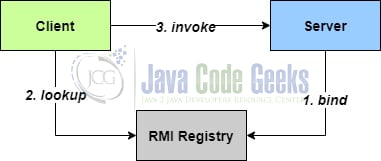
\includegraphics[height=100px]{JavaRMI.jpg}

Es gibt einen Server, der Objekte mittels bind/rebind unter einem gewissen Namen bei der RMI Registry veröffentlichen kann. Die Objekte, die der Server bei der RMI Registry veröffentlicht, müssen ein Interface implementieren, das vom Interface Remote erbt. Clients können über eine Methode lookup veröffentliche Objekte bei ihrem Namen in der RMI Registry finden und so Referenzen auf sie erhalten. Der Client kann dann die Methoden des Remote Interfaces auf dem Objekt aufrufen, wodurch der Code auf dem Rechner ausgeführt wird, der das Objekt veröffentlicht hat. Hier ist es ganz normal möglich Objekte als Parameter oder Rückgabewert zu benutzen. RMI überträgt also die Objekte mit dem Bytecode.\\
Mit RMI können z.B. auf einfache Weise Rechenservices implementiert werden, indem der Server ein Objekt mit einer Methode bereitstellt, die ein beliebiges Objekt übernimmt, einen in dem übergeben Objekt definierten Taks ausführt, und den Rückgabewert zurückgibt. Der Client kann dann die Methode des Server-Objektes mit seinen eigenen Objekten, also Tasks, als Argumente aufrufen.\\

\textbf{Fazit:} Bei OoM wird von Client und Server initial die IP-Adresse des Brokers benötigt. Sonst brauchen Server und Client aber keine Kenntnis darüber haben, wo sich ihre Kommunikationspartner befinden und wie viele es gibt. Daher ist OoM verteilungstransparent. Der Zugriff auf Ressourcen wird durch OoM ebenfalls sehr einfach.

\subsection{Web Services}
\subsubsection{SOAP, UDDI, WSDL}

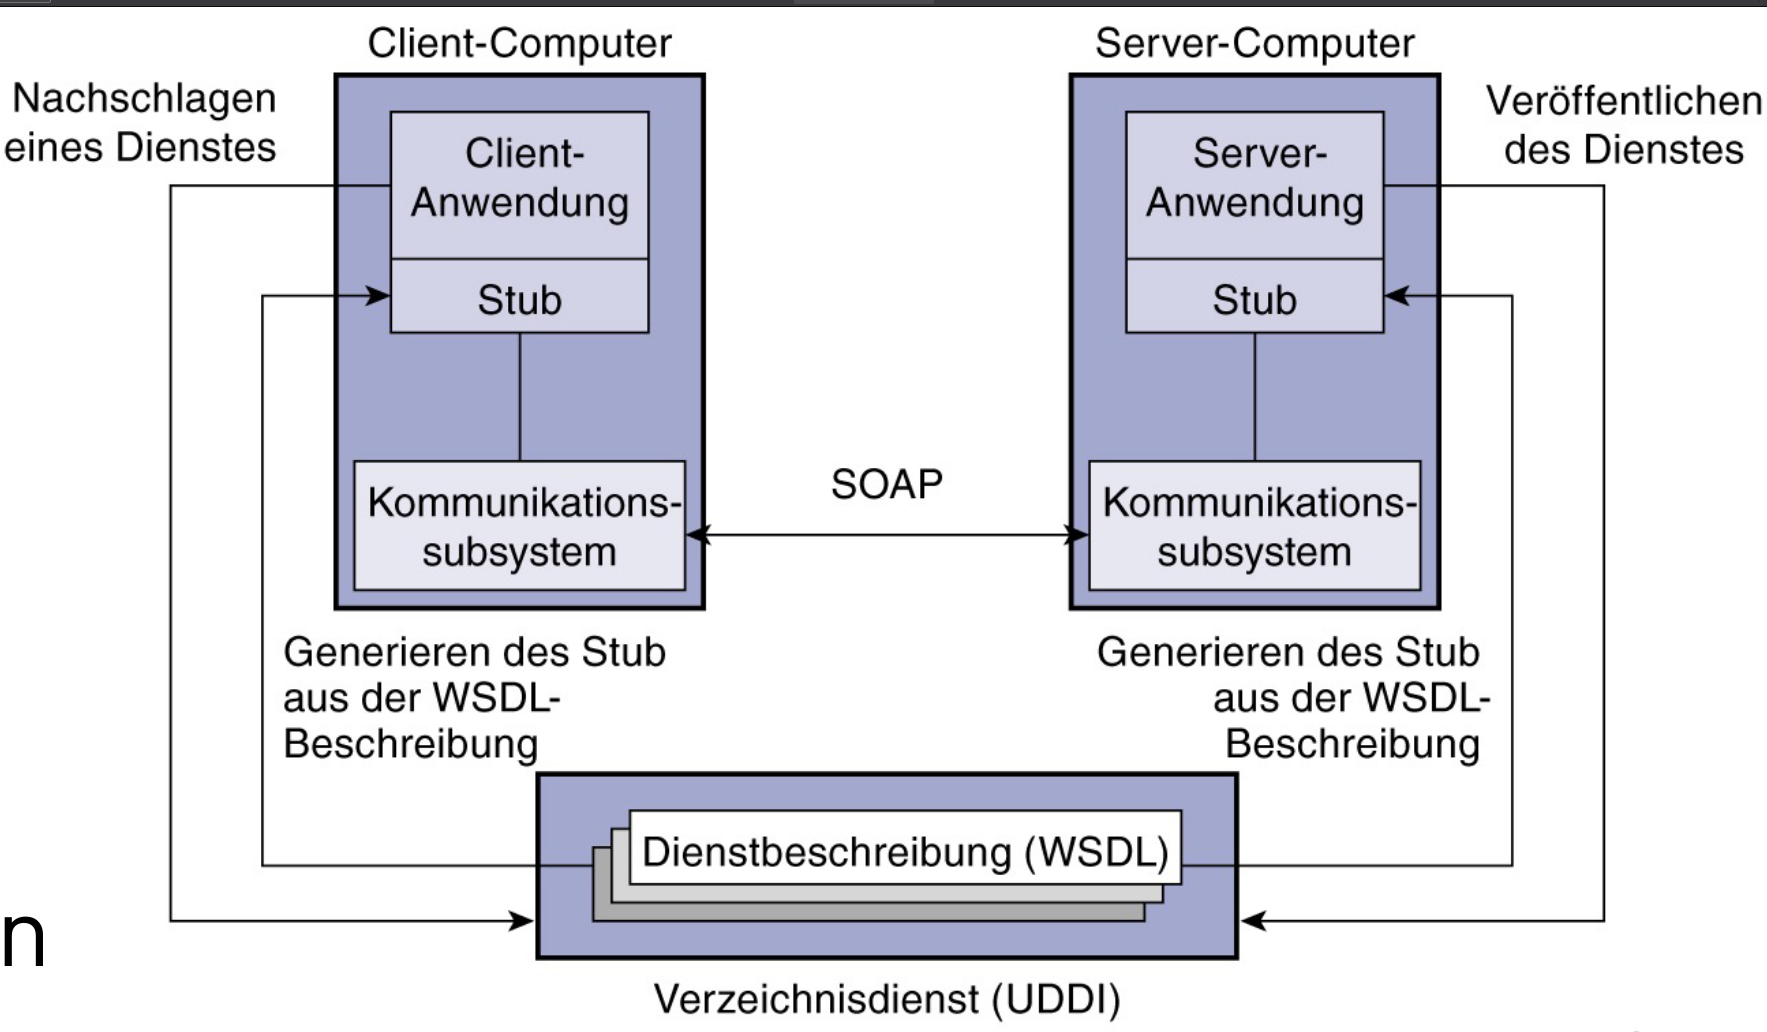
\includegraphics[height=200px]{SOAP.png}

SOAP steht für Simple Object Access Protocol und ist ein XML basiertes Protokoll zur Bereitstellung von Webservices, das gewöhnlich HTTP als Trägerprotokoll nutzt.\\
Die wesentlichen Dinge, die in einer Infrastruktur, die SOAP nutzt, wichtig sind, sind  WSDL (Web Service Definition Language) und UDDI (Universal Description, Discovery and Integration).\\
Die Beschreibungssprache WSDL wird genutzt, um zu definieren welche Funktionalitäten ein Webservice bereitstellt. Diese Schnittstellenbeschreibung wird auf einem Verzeichnisdienst, der UDDI-Registry, hinterlegt. Aus der WSDL können direkt sog. Stubs generiert werden. Das sind generierte Funktionen oder Klassen in einer bestimmten Programmiersprache, z.B. Java, die von Anwendungen benutzt werden können und SOAP implementieren. SOAP selbst ist ein XML-basiertes Protokoll in dem Anfragen und Antworten an/von den Services kodiert werden können. Das ist also ähnlich wie bei RPC-Frameworks, wo auch aus einer gemeinsamen Schnittstellenbeschreibung Code für Server und Client generiert wird.\\
Die Veröffentlichung einer WSDL Beschreibung und das auffinden dieser verläuft über die die UDDI-Registry. Die Kommunikation selbst verläuft dann aber ohne Umweg zwischen Client und Server.

\textbf{Fazit:}
UDDI bringt eine gewisse Ortstransparenz, da Client und Server nur die Schnittstelle über die UDDI-Registry erfahren müssen und dann ohne wissen über den Standort miteinander kommunizieren können.

\subsubsection{REST}

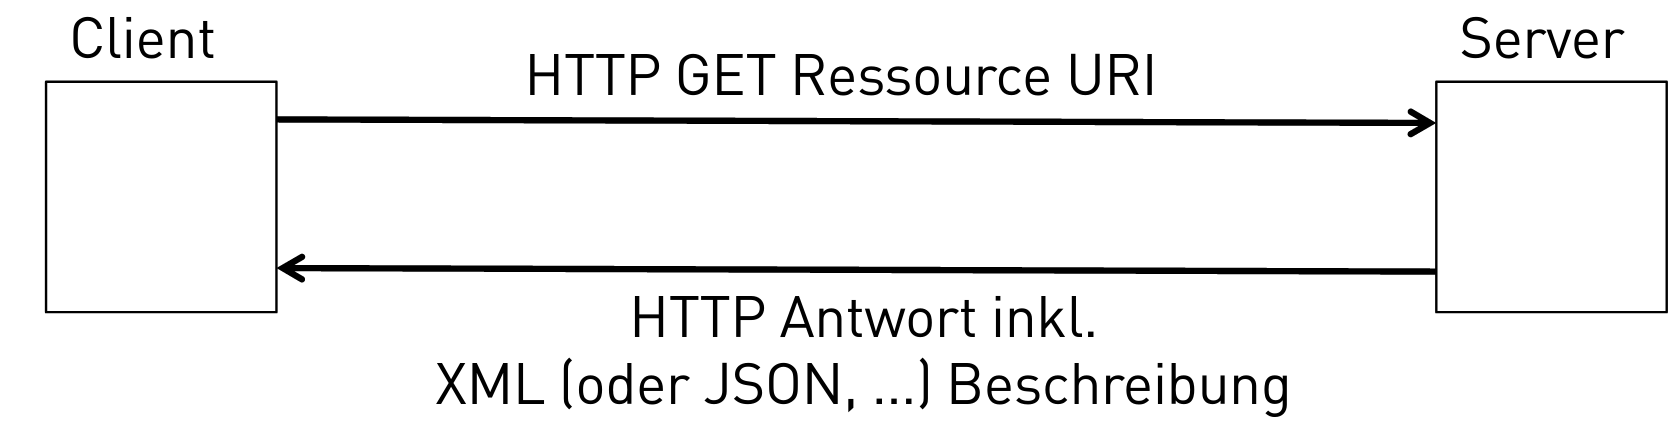
\includegraphics[height=80px]{REST.png}

REST (REpresentational State Transfer) kommt ursprünglich aus einer Doktorarbeit von Roy Fielding im Jahr 2000. Dort hat er beschrieben, wie alle CRUD Operationen eines Web-Services mittels HTTP GET, POST, PUT, PATCH, DELETE durchgeführt werden sollen können. Die Parameter und die Rückgabewerte werden in einem standardisierten XML-Format kodiert.\\
Heutezutage haben wir meist ein etwas anderes Verständnis von REST. REST ist inzwischen meist einfach eine Bezeichnung dafür, dass ein HTTP GET an eine bestimmte URL geschickt wird, die bestimmt was der Aufruf bewirken soll. Der Name des Services und die Parameter werden also in der URL kodiert. Falls es eine Antwort mit Daten gibt, wird sie oft in JSON kodiert.\\
Ein gutes Beispiel für eine URL, die auf eine REST API verweist ist:\\
https://api.twitter.com/1.1/statuses/mentions\_timeline.json?count=2\&since\_id=14927799\\
Hier werden z.B. recht offensichtlich die ersten 2 Stati seit der id=14927799 von der API verlangt.\\

\textbf{Fazit:}
REST ist sehr leichtgewichtig und einfach zu verstehen und umzusetzen. Es bietet einfachen Zugriff auf Ressourcen, sorgt jedoch nicht viel für Transparenz. Der Client muss dennoch den genauen Namen des Servers und die URLs seiner bereitgestellten Services kennen. Ein Fortschritt in der Transparenz ist jedoch, dass der Client nur noch den Hostnamen des Servers kennen muss und sich nicht mehr um Ports kümmern muss, da der Port 80 implizit angenommen wird. Da REST mit einfachen Mitteln gebaut ist liefert es auch Offenheit.
\section{Replikation}

\subsection{Was ist Replikation?}

Replikation bedeutet im Bezug auf verteilte Systeme, dass wir einen Service mehrfach d.h. auf mehreren Rechnern anbieten. Wenn der Service mit Daten arbeitet müssen folglich auch die Daten mehrfach vorhanden sein. Replikation kann die Verfügbarkeit eines Systems erhöhen und konkret bei folgenden Punkten hilfreich sein:

\begin{itemize}
    \item \textbf{Latenzoptimierung:} Services wie ein Webserver können repliziert in verschiedenen Teilen der Welt aktiv sein. Damit kann ein Client sich mit dem zu ihm nächsten Server verbinden und somit die Latenz senken. Es gibt Anbieter, die solche Arten von Rechnern vermieten, damit Kunden ihre Server an vielen Orten gleichzeitig hosten können.
    \item \textbf{Lastverteilung \& Skalierbarkeit:} Wenn ein die Nachfrage nach einem Service zu hoch wird kann manchmal ein einzelner Rechner nicht mehr ausreichen. Der Service muss repliziert werden, damit alle Anfragen bewältigt werden können. Bei Webservern ist es typisch, dass so viele Anfragen gesendet werden, sodass ein Server nicht mehr gut damit umgehen kann. Es gibt auch Services, bei denen zwar nicht viele Anfragen eintreffen, aber jede Anfrage dermaßen viel CPU power erfordert, dass die Aufgabe an mehrere replizierte Rechner verteilt werden muss.
    \item \textbf{Fehlertoleranz \& Ausfallsicherheit:} Wenn es mehrere Rechner gibt, welche den gleichen Service anbieten, kann im Falle eines Ausfalls der defekte Server ersetzt werden.
\end{itemize}


Wenn wir das \hyperref[sec:CAP_Theorem]{Cap Theorem} betrachten, merken wir, dass Replikation uns bei Partition Tolerance und Availability helfen kann. Allerdings steht Replikation in Konflikt mit Consistency, da durch redundante Datenspeicherung Inkonsistenzen entstehen können. Somit spielt das Thema Synchronisation auch eine große Rolle im Zusammenhang mit Repliklation.

\subsection{Implementierungsmodelle für Replikation}
In diesem Kapitel wollen wir einige Implementierungsmodelle ansehen, die Replikation benutzen.

\subsubsection{Caching}
Caching ist auch ein Verfahren der Replikation. Das Prinzip ist einfach. Wenn ein Client Daten über ein Netzwerk abgefragt hat, dann speichert er diese Daten für eine gewisse Zeit in einem lokalen Speicher, dem Cache. Wenn er später diese Daten erneut haben möchte, so kann er sie aus seinem Cache laden und so die Transferzeit über das langsamere Netzwerk einsparen. Schwierigkeiten treten auf, wenn sich die Daten ändern und dadurch die Daten des Caches veraltet sind.

\subsubsection{Fail-Over-Cluster}
\label{sec:fail-over-cluster}

Unter einem Fail Over Cluster versteht man ein System, in dem für einen bestimmten Server ein Backup Server bereit steht. Das heißt falls der eigentliche Server ausfällt, können alle Anfragen auf den Replikatserver umgeleitet werden. Wir unterscheiden zwischen zwei Typen von Fail-Over Implementierungen:
\begin{enumerate}
    \item \textbf{Hot Stand-By}: Der Replikatserver steht immer bereit
    \item \textbf{Cold Stand-By}: Der Replikatserver ist nur physisch vorhanden und muss im Einsatzfall noch gebootet werden.
\end{enumerate}

Fail-Over Cluster bieten Ausfallsicherheit, bieten jedoch nicht mehr Verfügbarkeit oder Skalierbarkeit. Außerdem werden die Hardwareressourcen schlecht genutzt, da im Normalfall (d.h. nicht Fehlerfall) nur der Hauptserver aktiv ist.

\subsubsection{Server Cluster - Klassisch}
\label{sec:classic-server-cluster}

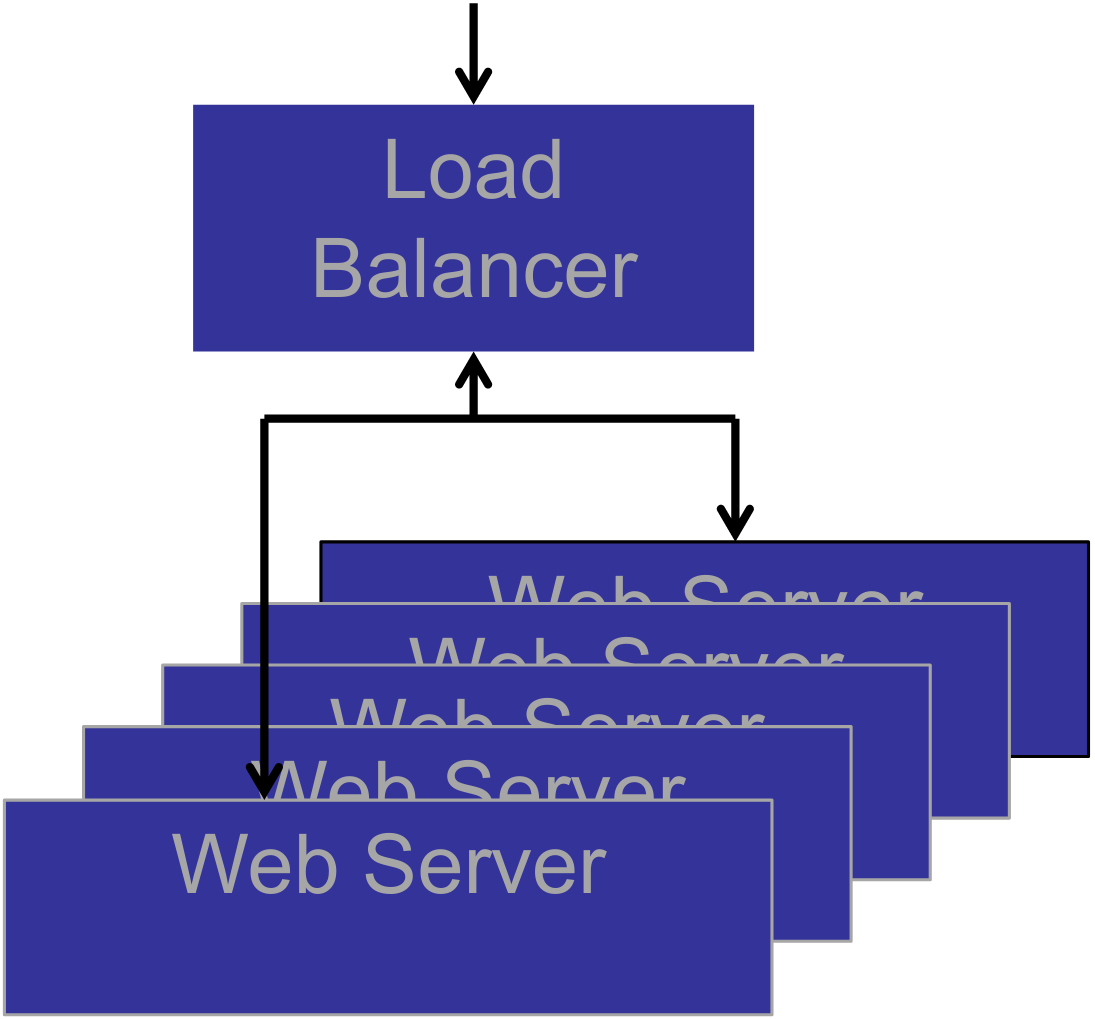
\includegraphics[height=150px]{ClusterMitLoadBalancer.png}

In dieser Architektur haben wir eine Vielzahl von gleichwertigen Servern, auf die Aufgaben verteilt werden können. Anfragen werden zunächst immer an einen Vermittler, den Load-Balancer, geschickt. Dieser entscheidet dann mittels eines simplen Verfahrens (z.B. Round-Robin), welcher Server des Clusters die Anfrage bearbeiten soll. Dadurch wird der Rechner, an den die Anfragen gesendet werden, entlastet. Dennoch werden alle Anfragen von nur einem Rechner bearbeitet, sodass dieser zum Bottleneck werden kann. Eine Möglichkeit das zu bewältigen sehen wir im Kapitel über \hyperref[client-based]{Client-Basierte Verfahren}. Außerdem ist das Gesamtsystem lahmgelegt, wenn bloß der Load Balancer ausfällt. Das kann einfach bewältigt werden, indem ein \hyperref[sec:fail-over-cluster]{Fail-Over-Cluster} für den Load-Balancer eingerichtet wird.\\
Ein weiteres Problem entsteht, wenn von den Clustern des Servers auch Daten geschrieben werden sollen. Dann müssten sofort die Daten auf den anderen Servern synchronisiert werden, um die Konsistenz beizubehalten.

\subsubsection{Server Cluster - n-Tier-Architektur}

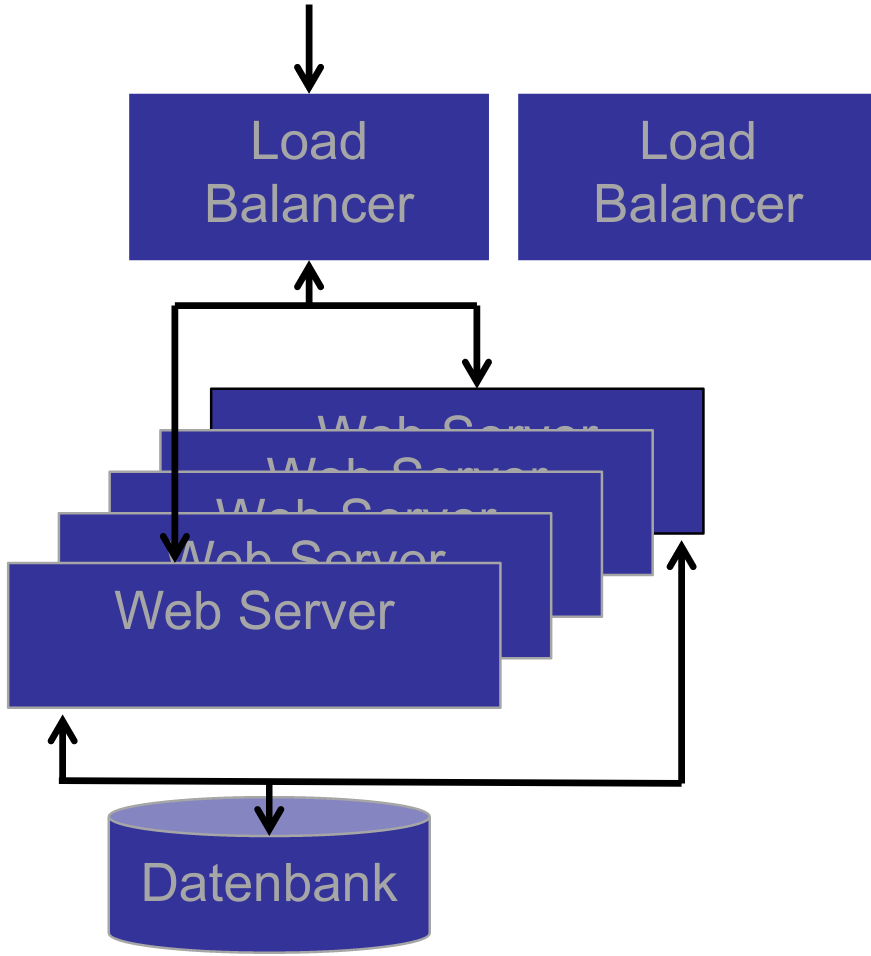
\includegraphics[height=150px]{n-tier-architektur.png}

Bei einer n-Tier-Architektur wir in der untersten Schicht mit einer gemeinsamen Datenquelle gearbeitet, um inkonsistenzen zu vermeiden. Somit sind, im Gegensatz zu einem \hyperref[sec:classic-server-cluster]{klassischen Server-Cluster}, auch Schreibzugriffe ohne inkonsistenzen möglich. Allerdings kann so die DB zum Bottleneck werden, weshalb viele DBMS schon von sich aus eine intelligentes Clustering implementieren.

\subsubsection{Server Cluster - Master-Slave}
\label{sec:master-slave}

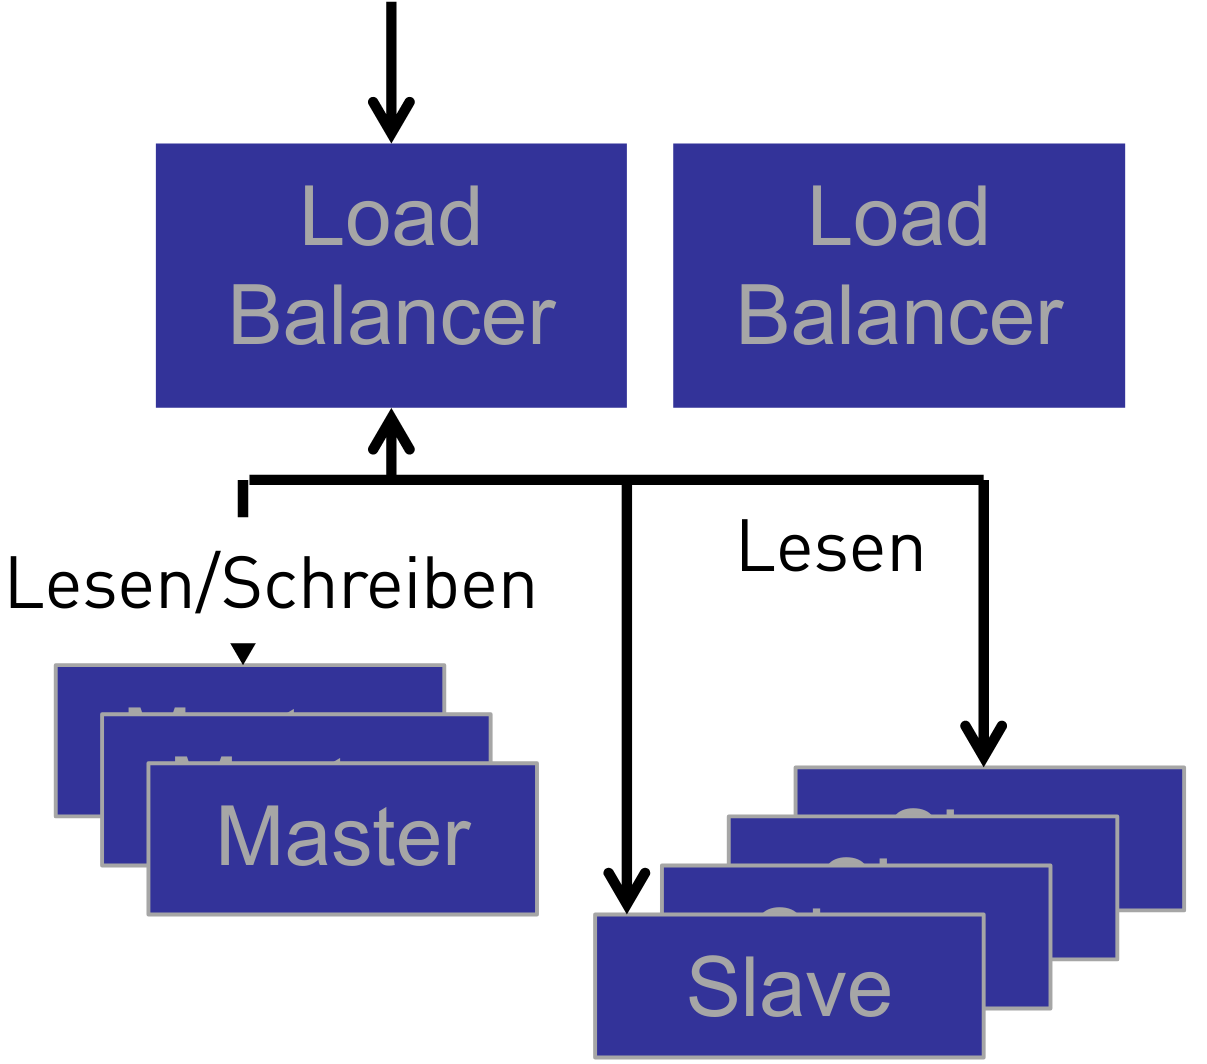
\includegraphics[height=150px]{MasterSlave.png}

In vielen Systemen sind Lesezugriffe deutlich häufiger als Schreibzugriffe. Dann bietet sich eine Master-Slave-Architektur an. Es gibt Master, die lesen und schreiben dürfen und Slaves, dei nur lesen dürfen. Wenn eine Master Daten verändert, dann sorgt er dafür, dass die Daten mit den Slaves synchronisiert werden. Auf diese Weise kann die Kommunikation zwischen den replizierten Servern verringert werden, da bekannt ist an welchen Knotenpunkten sich Daten ändern können.

\textbf{Verteilte Mater-Slaves:}\\
Eine andere Implementierungsvariante ist, dass jeder Server ein Master mit exklusivem Schreibzugriff für einen Bestimmten Teil der Daten ist. Auf diese Weise kann es zu keinen Schreib-anomalien mehr kommen, da in jedem Fall der eine schreibende Master der einzige ist, der diese Daten schreibt und damit die Daten auf diesem Master immer aktuell sind. Dennoch muss der Master nach einem Schreibzugriff die Daten auf die anderen Server verteilen, damit die Lesezugriffe von dort aus konsistent sind. Verteilte Mater-Slave Architekturen sind besonders skalierbar, da die Daten in beliebig viele Partitionen aufgeteilt werden können.

\textbf{Hashing:}
Die Load-Balancer müssen wissen auf welchen Server eine Anfrage umgeleitet werden soll. Das kann recht einfach mit Hash-Funktionen geschehen. Z.B. könnte man sich den Zugriff auf eine DB mit einem Primärschlüssel von integralem Typ vorstellen. Dann könnte eine Hashfunktion eine ID dieser DB mittels Modulo n auf n gleich große Gruppen aufteilen.



\subsubsection{Client-basierte Verfahren}
\label{client-based}

Wir können uns auch den Load-Balancer in einem \hyperref[sec:classic-server-cluster]{klassichen Server Cluster} sparen, indem wir die nötige Verteilungslogik in den Clients implementieren. Wenn z.B. jeder Client die Adresse aller Server, die einen Dienst anbieten, kennt, kann er einen zufälligen Server aussuchen, um so die Serverlast zu verteilen.\\
Eine mögliche Implementierung kann mithilfe von DNS SRVs (Service Records) erfolgen. In diesen Records können für einen Service die IP-Adressen aller Server eingetragen werden, die ihn anbieten. Dieses Verfahren wird z.B. beim SIP Protokoll für Voice-Over-IP verwendet.

\subsubsection{Map-Reduce-Verfahren}
\label{sec:map-reduce}

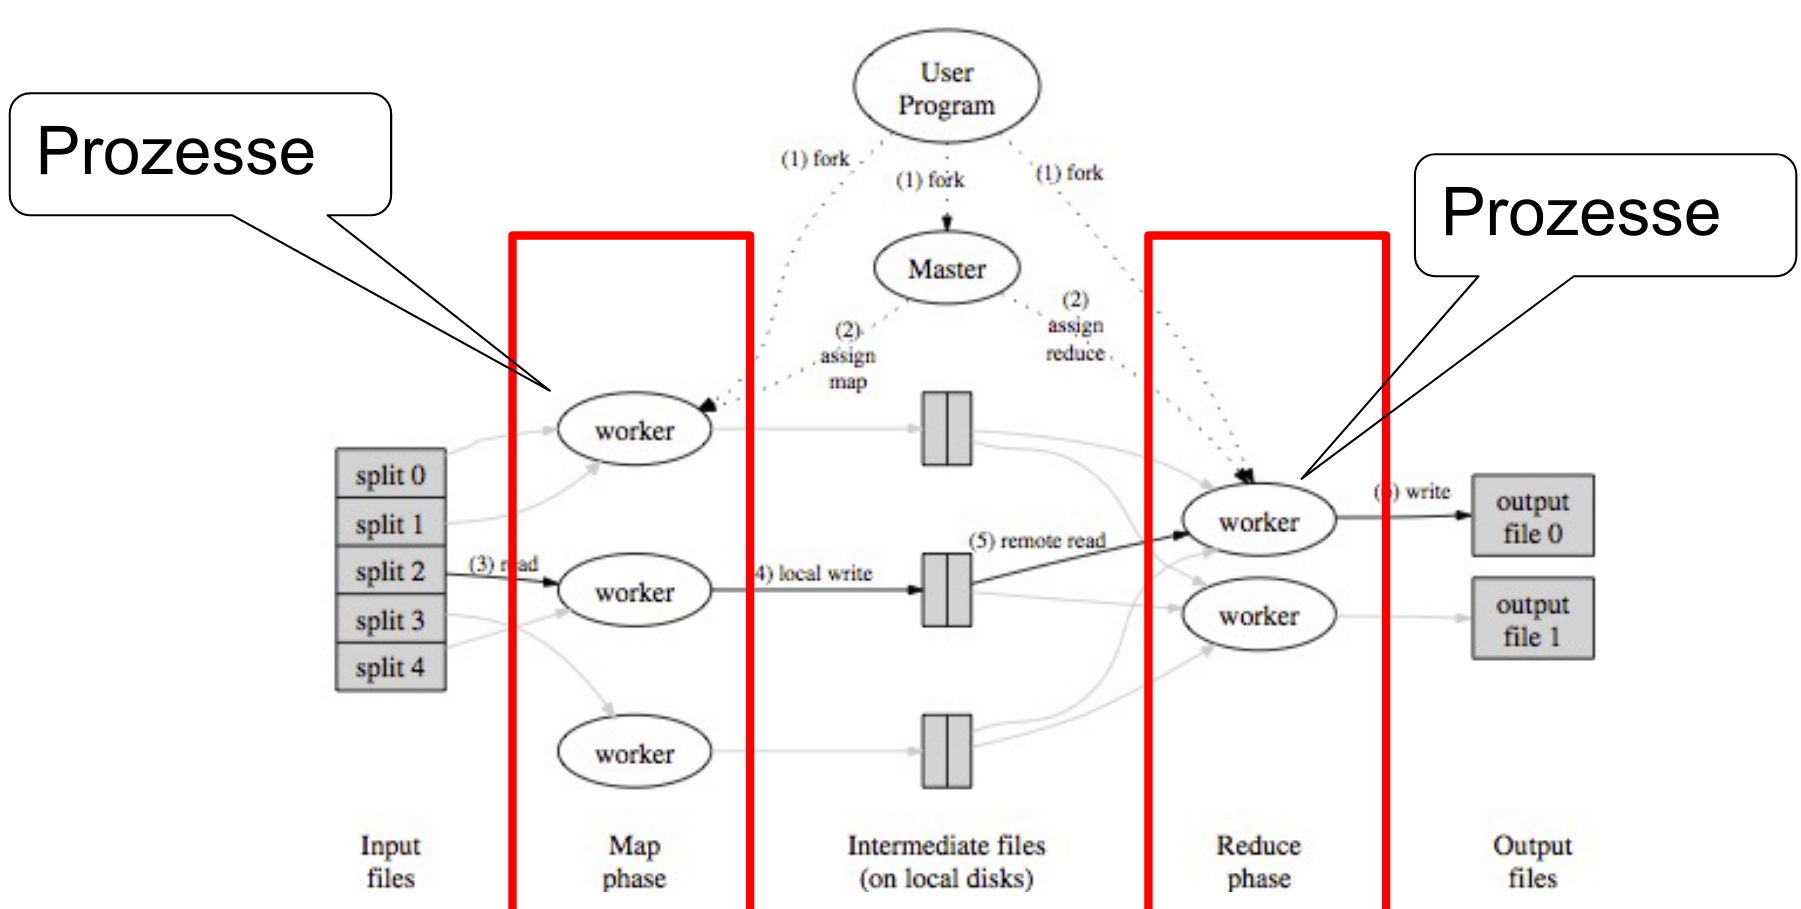
\includegraphics[height=200px]{map-reduce.png}

Map-Reduce ist ein von Google entwickeltes Verfahren zur Lastaufteilung bei CPU-intensiven Operationen. Das heißt hier geht es nicht darum möglichst viele Anfragen zu bewältigen, sonder eine Anfrage, die unglaublich viel Rechenpower benötigt, parallel auszuführen.\\
Bei diesem Verfahren werden die Eingangsdaten in gleichartige, ungefähr gleich aufwendige Pakete unterteilt. Jedes Paket wird an einen Worker verteilt. Die Worker machen den Job, der im Anwendungskontext, ausgeführt werden soll und verpacken das Ergebnis in key-value-Paare (map-phase). Dabei entstehen die sogenannten intermediate files, die dann in der reduce phase von separaten Prozessen zu einem Gesamtergebnis akkumuliert werden sollen.\\
Dieses Verfahren ist sehr einfach und unbegrenzt skalierbar. Allerdings ist es auch nur für eine bestimmt Gruppe von Problemen anwendbar. Nämlich für solche, bei denen ein Problem in unabhängige Teilprobleme, also solche bei denen keine Kommunikation zwischen den Workern notwendig ist, unterteilt werden kann. Zusätzlich muss es möglich sein, die Teilergebnisse als Key-Value Paare darzustellen und diese dann zu akkumulieren. Die Logik in der Map- und Reduce-Phase muss also gut durchdacht sein. Ein Anwendungsbeispiel ist etwa bei Suchmaschinen das durchsuchen vieler Millionen Texte nach einem Schlüsselwort. Jeder Worker übernimmt dann eine bestimmte Anzahl von Texten. Das Ergebnis der Map-Phase sind einzelne key-value-Paare, die z.B. aus der URL zum durchsuchten Text und der Häufigkeit des gesuchten Wortes bestehen. In der Reduce-Phase wäre in diesem Fall nicht mehr zu tun als die Ergebnisse der Map-Phase gesammelt zurückzugeben.\\

Dienste, die Map-Reduce anbieten, sind z.B.:
\begin{itemize}
    \item Amazon Elastic Map Reduce
    \item Google App Engine
    \item Bibliothek: Apache Hadoop
\end{itemize}

\textbf{Variante: Apache Spark}\\
Apache Spark ist eine Open-Source-Lib, die darauf ausgelegt ist, mehrere iterationen von Map-Reduce hintereinander durchzuführen. Dabei können die Ergebnisse der einzelnen Iterationen im HS zwischengespeichert werden und von den nächsten Iterationen abgerufen werden. Verglichen mit klassischem Map-Reduce (z.B. Hadoop) ist Spark je nach Anwendungsfall möglicherweise deutlich schneller. Allerding können in Hadoop deutlich größere Datenmengen verarbeitet werden, da die Daten über das Dateisystem geladen werden.


\subsection{Pipelining \& Interner Serveraufbau}

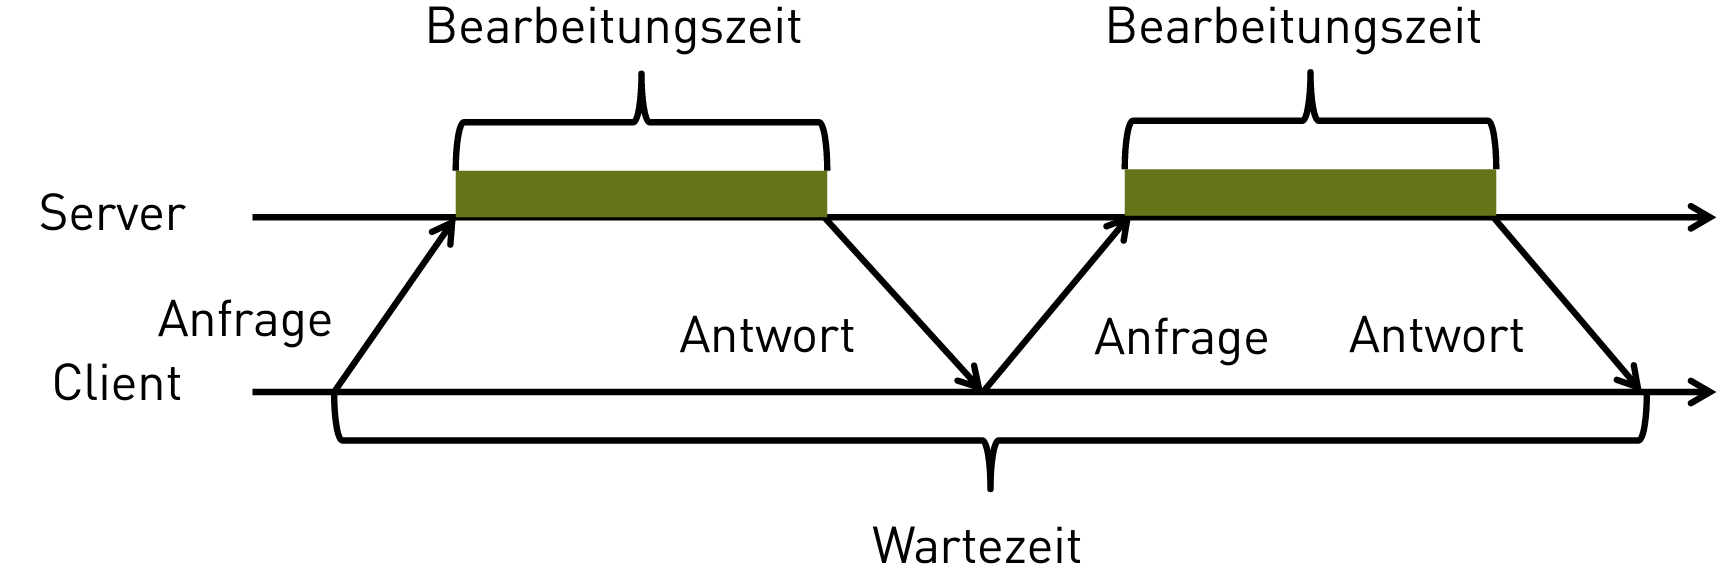
\includegraphics[width=300px]{pipelining1.png}

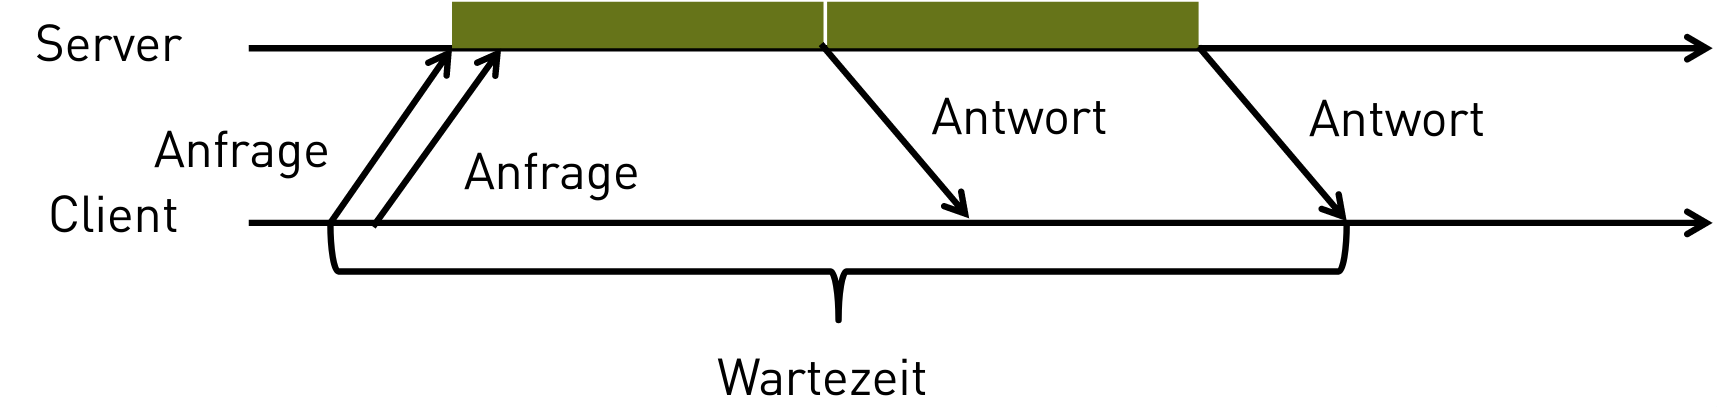
\includegraphics[width=300px]{pipelining2.png}

Im oberen Bild können wir sehen, dass der Client nach dem Senden einer Nachricht auf die Antwort wartet und dann erst die zweite Anfrage sendet. Manche Protokolle (z.B. Http 1.1) unterstützen aber auch die Möglichkeit mehrere Anfragen zu schicken ohne auf die Antwort der vorherigen Anfrage zu warten. Auf diese Weise hat der Server weniger Leerlauf und die Antworten treffen mit weniger Wartezeit beim Client ein.\\

Intern arbeiten die Server allerdings auch oft mit mehreren Threads. Ist das der Fall, so muss Pipelining nicht mehr beachtet werden, da jede Anfrage ohnehin von einem anderen Thread behandelt wird.
\section{Zeiten}

\subsection{Physikalische Zeit}

\subsubsection{Physikalische Zeit auf verschiedenen Rechnern}
Die physikalische Zeit stellt die uns im Alltag bekannte Uhrzeit dar. Die physikalische Zeit ist in vielen kryptographischen Verfahren von Bedeutung, da z.B. bestimmte Zertifikate (z.B. TSL) oder Authentifizierungen nur in einem bestimmten Zeitraum gültig sind. Deshalb ist ein genaues und sicheres Verfahren zur Bestimmung der physikalischen Zeit erwünscht.\\
Die physikalische Zeit, die wir auf einem Rechner haben wollen, ist die \textbf{Universal Time Coordinated (UTC)}, die auf internationaler Atomzeit basiert. Sie wird Weltweit über Kurzwelle oder Satellit ausgestrahlt. Aus der UTC kann man selbstverständlich die lokale Zeit errechnen.\\
Um sicherzustellen, dass jeder Rechner (oder andere Devices wie Smartphones oder IoT-Geräte) Zugriff zur UTC hat ist es naheliegend jeweils einen Atomzeitempfänger einzubauen. Da diese Empfänger aber zu teuer sind möchte man stattdessen nur wenige (spezielle) Rechner damit ausstatten und von dort aus die Zeit an alle anderen Rechner verteilen. Das Problem, dass sich ergibt, ist, dass Uhren in Rechnern nicht absolut genau laufen und deshalb periodisch synchronisiert werden müssen. Es stellt sich nun die Frage, wie ein Rechner damit umgehen soll, wenn er bei der Synchronisation feststellt, dass seine lokale Uhrzeit abgedriftet ist, also nichtmehr stimmt:
\begin{itemize}
    \item \textbf{lokale Uhr hängt hinterher:} In diesem Fall kann die lokale Zeit sofort angepasst werden und alle Events, die in dem übersprungenen Intervall gescheduled waren, werden sofort ausgeführt.
    \item \textbf{lokale Uhr ist zu weit:} In diesem Fall können wir die Uhr nicht zurückstellen, da sonst möglicherweise Events, die in dem dazwischenliegenden Zeitintervall gescheduled, waren doppelt ausgeführt werden würden. Demnach muss die lokale Uhr verlangsamt werden, also einige Ticks ausgesetzt werden, um die Korrektur durchzuführen.
\end{itemize}

Eine weitere Frage, die sich stellt, ist, wie oft diese Synchronisation durchgeführt werden sollte. Üblicherweise gibt der Hersteller des Geräts einen Wert $\rho$ an, der die maximale Abweichung nach einer bestimmten Zeiteinheit angibt. Daraus folgt, dass 2 verschiedene Uhren dieses Herstellers nach $\Delta t$ Zeiteinheiten eine maximale Abweichung $\delta = 2 \rho \Delta t$ Zeiteinheiten haben (, wenn die Uhr des einen Rechners maximal langsam und die des anderen maximal schnell lief). Durch Umstellen der Gleichung ergibt sich
\[ \Delta  t = \frac{\delta}{2 \rho}\]

Wir können uns nun eine maximale Abweichung $\delta$ überlegen, die wir erlauben wollen. Durch das Einsetzten in die Gleichung erhalten wir die Zykluslänge der Synchronisationen, die benötigt wird, um diese maximale Abweichung nicht zu überschreiten.

\subsubsection{Uhrabgleich - Christian\textquotesingle s Algorithm}

Der Christian\textquotesingle s Algorithm ist eine sehr simple Möglichkeit mehrere Rechner mit einem zentralen Zeitserver (der z.B. ein Atomzeitempfänger ist) abzugleichen. Das Verfahren ist wie folgt:
\begin{itemize}
    \item Jeder Client fragt zyklisch den zentralen Server nach seiner Uhrzeit
    \item Beim eintreffen der Nachricht berechnet der Client die Round Trip Time (RTT).
    \item Der Client addiert zur empfangenen Zeit die Hälfte der  RTT, um die Zeit, die für den Transfer benötigt wurde, auszugleichen und passt seine eigene Uhr an (verlangsamen oder Zeit übernehmen)
\end{itemize}

\subsubsection{Uhrabgleich - Berkeley Algorithm}

Der Berkeley Algorithmus ist ein einfaches Verfahren, um die Uhren von mehreren Rechnern zu synchronisieren. Dabei gibt es keinen Atomzeitempfänger und keinen Anspruch auf das Benutzen der wahren UTC. Stattdessen wird nur sichergestellt, das alle Rechner untereinander die gleiche Zeit haben (welche auch immer das dann ist). Das Verfahren ist wie folgt:
\begin{itemize}
    \item Ein zentraler Server fragt alle anderen Rechner zyklisch nach ihrer lokalen Zeit
    \item Der Server ermittelt den Mittelwert der lokalen Zeiten und sendet ihn an alle Rechner
    \item Die Rechner passen ihre lokale Zeit an den Mittelwert an
\end{itemize}

\subsubsection{Problem: beim Berkeley und Christian\textquotesingle s Algorithmus - Offset mit RTT bestimmen}
\label{sec:offset-with-rtt}

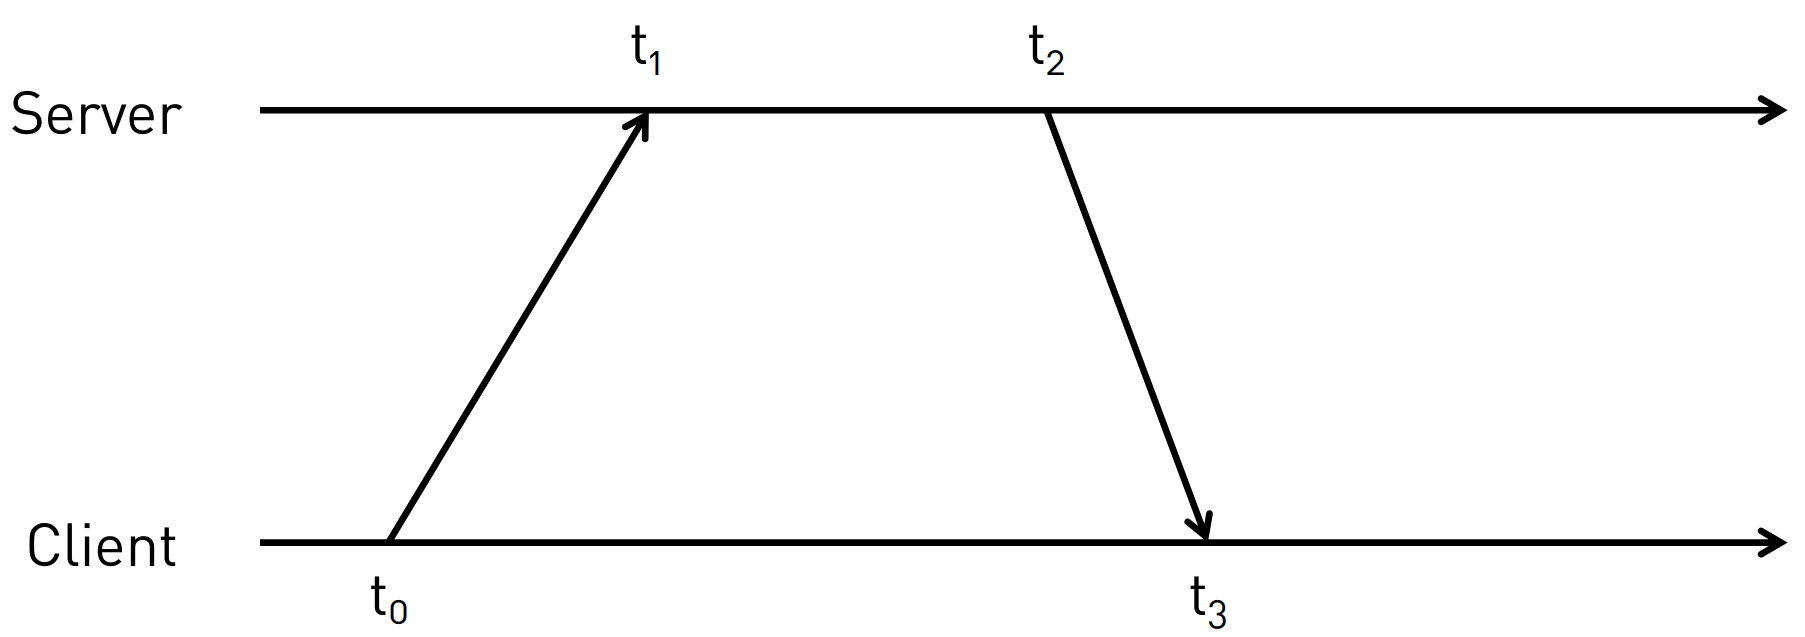
\includegraphics[height=130px]{RTT.png}

Wenn ein Rechner eine Zeit von einem Server gesendet bekommt, muss er beachten, dass diese schon wieder durch die Verzögerung des Netzwerks veraltet ist. Im Bild ist $t_{0}$ der Zeitpunkt an dem die Anfrage an den Zeitserver gesendet wird. Zum Zeitpunkt $t_{1}$ empfängt der Server die Anfrage und beantwortet sie zum Zeitpunkt $t_{2}$ mit der Zeit in diesem Moment. Der Client erhält diese Nachricht zu einem späteren Zeitpunkt $t_{3}$. Um die genaue Zeit auf dem Client zu bestimmen, müssten wir offensichtlich zur vom Server gesendeten Zeit die Übertragungszeit dieser Nachricht $\Delta t = t_{3} - t_{2}$ addieren. Das ist aber \textbf{nicht möglich}, da diese absoluten Zeiten von verschiedenen Uhren gemessen wurden und somit nicht vergleichbar sind. Stattdessen können wir nur jeweils die absoluten Zeiten $t_{0}$ und $t_{3}$, sowie $t_{1}$ und $t_{2}$ vergleichen. Somit können wir \textbf{nur näherungsweise} den Offset bestimmen:
\[
    O \approx \frac{t_{0} - t_{3} - (t_{2} - t_{1})}{2}
\]

\subsubsection{NTP - Network Time Protocol}

\vspace{5px}

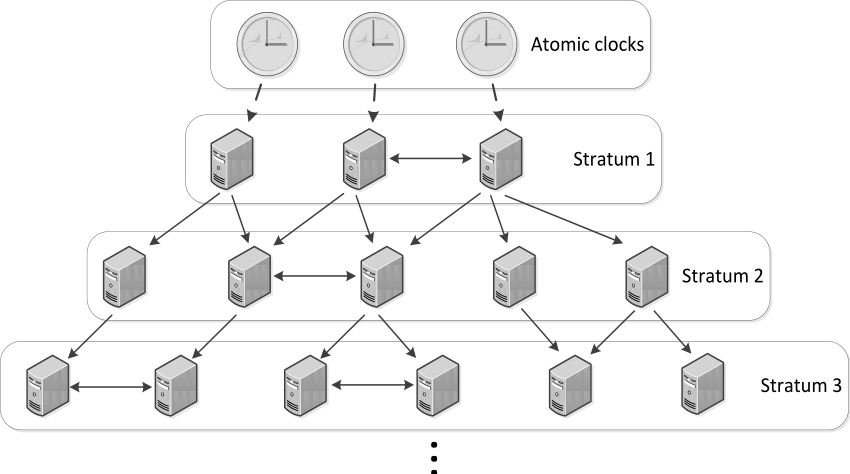
\includegraphics[height=170px]{NTP-typology.png}

Das Network Time Protocol (NTP) ist das Standardprotokoll zur Uhrensynchronisation im Internet. Dazu gibt es eine Reihe von Servern auf denen ein NTP-Daemon läuft. Die Topologie ist mehrschichtig in mehreren sogenannten Stratums aufgebaut, um skalierbar zu sein. Jeder Zeitserver aus Stratum $n$ ist ein Client (empfängt Zeit von Stratum $n-1$), ein Server (übermittelt Zeit zu Stratum $n+1$) und ein Peer (synchronisiert Zeit innerhalb Stratum $n$). Ein NTP-Daemon kann dabei auch mehrere Quellen abfragen und die \quotes{beste} Quelle wählen. Die Qualitätskriterien für Qualität eines Zeitservers könnte z.B. die RTT, sowie die Standardabweichung der RTT. Für der \hyperref[sec:offset-with-rtt]{Berechnung des Offsets} werden beim NTP immer mehrere Anfragen gestellt, und die ausgewählt, welche die kleinste RTT hat und somit die genauste Schätzung erlaubt.

\subsection{Logische Zeit}
\label{sec:logic-time}

Die logische Zeit definiert keine absolute Zeit, sonder lediglich eine Reihenfolge, in der Ereignisse stattfinden. Die Idee der logischen Zeit entsteht aus der Erkenntnis, dass es nicht immer notwendig ist die absolute Zeit zu kennen, sondern oft ausreicht, bestimmen zu können in welcher zeitlichen Ordnung Ereignisse aufgetreten sind.\\
Zunächst sollten wir uns fragen, welche Aussagen wir überhaupt über die Reihenfolge von Ereignissen in einem verteilten System treffen können. Wir werden feststellen, dass folgender Sachverhalt für Prozess P1 und P2 in einem verteilten System für die Relation "happened before" $\rightarrow$ gilt:
\begin{enumerate}
    \item Es kann eine totale Ordnung für lokale Ereignisse von Prozess P1 hergestellt werden, sodass für jedes Paar aus lokalen Ereignissen $x_{i_{P1}}$ und $x_{j_{P1}}$ gilt $x_{i_{P1}} \rightarrow x_{j_{P1}}$ oder $x_{j_{P1}}\rightarrow x_{i_{P1}}$
    \item Ist $x_{s_{P1}}$ ein Sendeereignis einer Nachricht des Prozesses P1 und $x_{r_{P2}}$ ein Empfangsereignis des Prozesses P2, so gilt in jedem Fall $x_{s_{P1}} \rightarrow x_{r_{P2}}$
    \item Über zwei Ereignisse $x_{i_{P1}}$ und $x_{j_{P2}}$ unterschiedlicher Prozesse kann ohne Zusatzinformationen keine Aussage bezüglich der Relation $\rightarrow$ getroffen werden. In solchen Fällen schreiben wir $x_{i_{P1}} || x_{j_{P2}}$, um zu zeigen, dass diese Ereignisse in keiner Relation stehen.
\end{enumerate}

Damit definiert die Relation $\rightarrow$ eine partielle Ordnung (Halbordnung) auf der Menge der Ereignisse auf Rechnern in einem verteilten System.\\

Eine wünschenswerte definition von logischer Zeit sollte allerdings eine totale Ordnung definieren, sodass für auch für unabhängige Ereignisse verschiedener Prozesse (siehe Punkt 3) eine Ordnung feststellbar ist. Um dies zu erreichen, können wir jedem Rechner eine eindeutige ID zuweisen und definieren, dass ein Ereignis nach seiner ID geordnet wird, falls die partielle Ordnung $x_{i_{P1}} || x_{j_{P2}}$ ergeben würde. Auf diese Weise können wir eine totale Ordnung erschaffen, was bedeutet, dass jeder Prozess eine Menge von Ereignissen (z.B. auch eine Menge von Nachrichten) auf genau die selbe Weise ordnet. Allerdings ist diese totale Ordnung künstlicher Natur, wenn wir nach der ID entscheiden, so geschieht dies zwar einheitlich, allerdings \textbf{können wir nicht sagen, ob Ereignisse, die nach der ID geordnet wurden tatsächlich in dieser Reihenfolge in der physikalischen Zeit eingetreten sind}.\\

Im Folgenden wollen wir Umsetzungen von Mechanismen zur Bestimmung partieller Ordnungen in verteilten Systemen kennenlernen (die natürlich zu künstlichen totalen Ordnungen gemäß unserer obigen Erkenntnis erweitert werden können).

\subsubsection{Lamport-Time}
\label{sec:lamport-time}

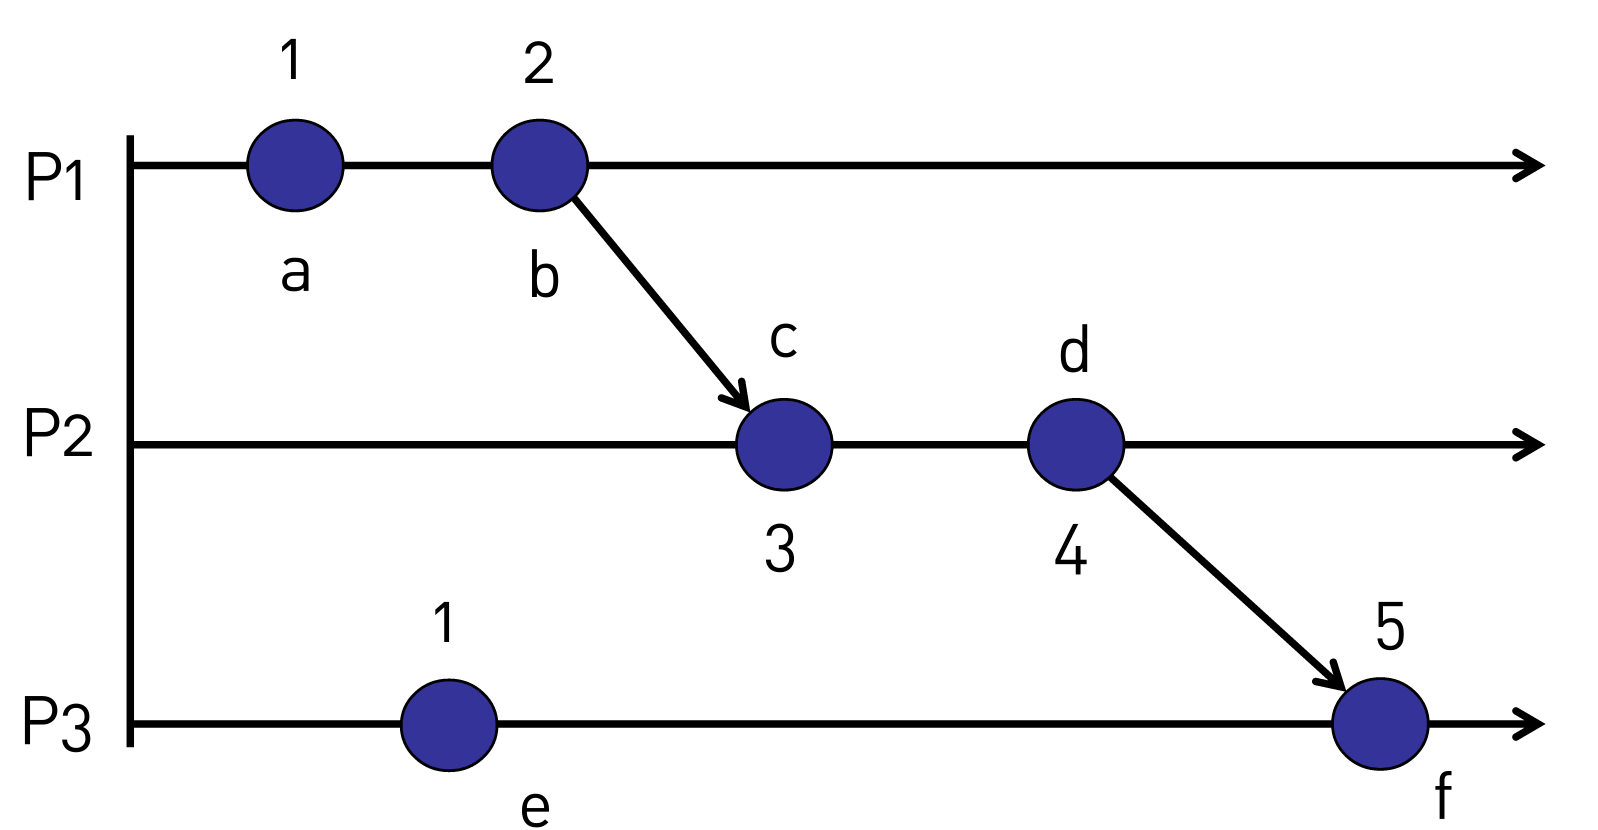
\includegraphics[height=180px]{LamportTime.png}

Die Lamport-Time speichert für jedes Ereignis $e$ einen Integer $L(e)$ , sodass $L(e_{i}) < L(e_{j})$ gilt, falls die Relation "happend before" $e_{i} \rightarrow e_{j}$ gilt. Andersherum gilt aber \textbf{nicht}, dass, wenn $L(e_{i}) < L(e_{j})$ gilt auch $e_{i} \rightarrow e_{j}$ gilt. Die Lamport-Time bildet also die partielle Ordungsrelation  $\rightarrow$ nur korrekt ab, ist aber nicht äquivalent zu ihr. Es gilt also:

\begin{align*}
    e_{i} \rightarrow e_{j} \qquad \Rightarrow \qquad  L(e_{i}) < L(e_{j})         \\
    L(e_{i}) < L(e_{j}) \qquad \cancel{\Rightarrow} \qquad e_{i} \rightarrow e_{j} \\
    e_{i} \rightarrow e_{j} \qquad \cancel{\Leftrightarrow} \qquad L(e_{i}) < L(e_{j})
\end{align*}

Konkret wird die Lamport-Time durch folgende Regeln umgesetzt:
\begin{enumerate}
    \item Zu Beginn stehen alle Zähler für Ereignisse auf 0
    \item Lokale Ereignisse (das schließt Sendeereignisse mit ein) bekommen als Zeit das Inkrement der  Lamport-Time ihres lokalen Vorgängers:\\
          $L(e_{i_{P1}}) = L(e_{i - 1_{P1}}) + 1$
    \item Mit Nachrichten wird die Lamport-Time des zugehörigen Sendeereignisses mitgeschickt
    \item Empfangsereignisse bekommen das Inkrement des Maximums der Lamport-Time ihres lokalen Vorgängers und der Lampert-Time der empfangenen Nachricht:\\
          $L(e_{i_{P1}}) = max(L(e_{i - 1_{P1}}), L(e_{n})) + 1$
\end{enumerate}

\subsubsection{Vector-Time}
\label{sec:vector-time}

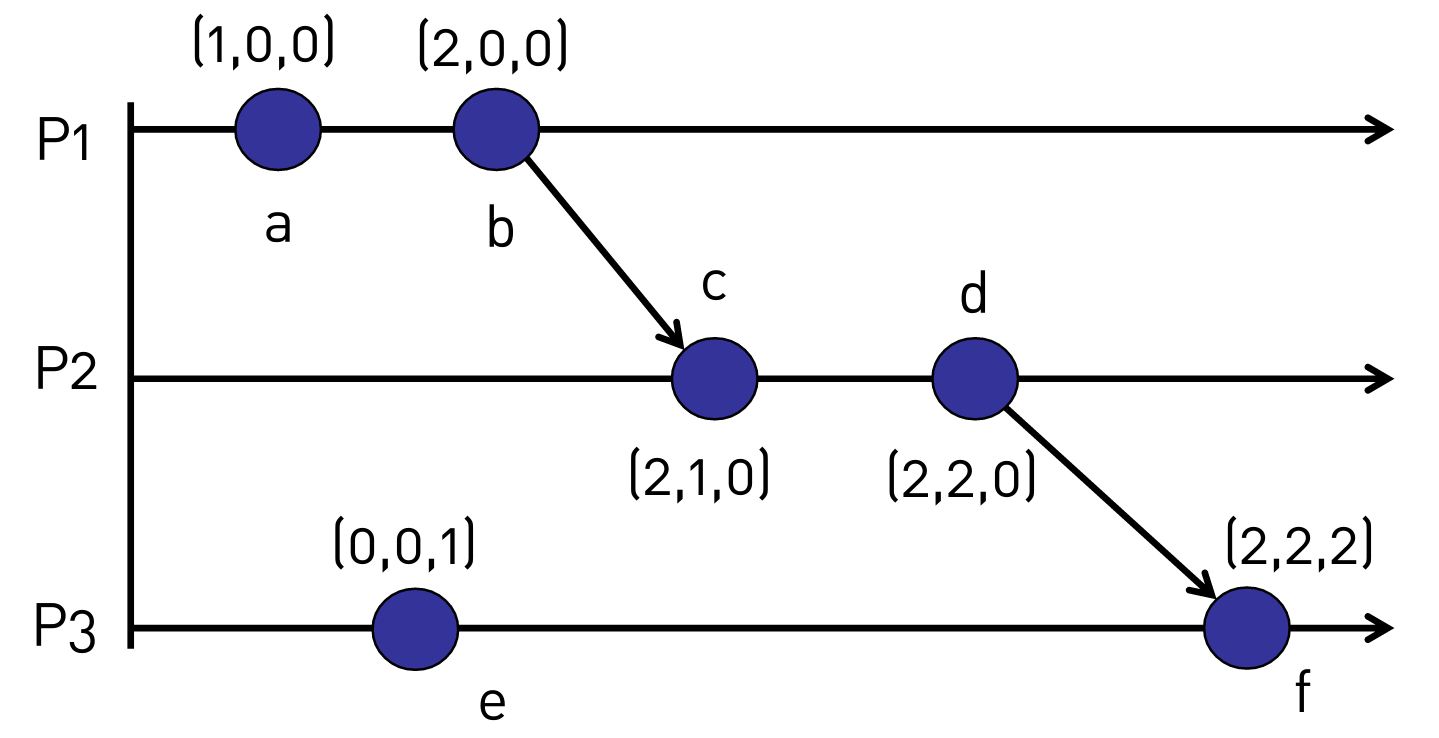
\includegraphics[height=180px]{VectorTime.png}

Die Vector-Time verbessert die \hyperref[sec:lamport-time]{Lamport-Time}, sodass eine kleiner-Relation $<$  über der Menge von Vector-Times äquivalent zur "happened-before"-Relation $\rightarrow$ der Ereignisse ist:
\begin{align*}
    V(e_{i}) < V(e_{j}) \qquad \Leftrightarrow \qquad e_{i} \rightarrow e_{j} \qquad \qquad \qquad \qquad \qquad \qquad \\
    V(e_{i}) = V(e_{j}) \qquad \Leftrightarrow \qquad (V(e_{i}) \quad \cancel{<} \quad V(e_{j})) \quad \wedge \quad (V(e_{j}) \quad \cancel{<} \quad V(e_{i})) \qquad \Leftrightarrow \qquad e_{i} \quad || \quad e_{j}
\end{align*}

Um dies zu erreichen wird für jedes Ereingnis $e$ nicht nur ein Integer gespeichert, sondern ein Vektor von Integern der Dimension $n$, wobei $n$ die Anzahl der Knoten im verteilten System ist und jede Komponente des Vektors einem Knoten zugeordnet wird.\\
Die Kleiner-Relation $<$ ist so, definiert, dass $V(e_{i}) < V(e_{j})$ genau dann gilt, wenn alle Komponenten von $V(e_{i})$ kleiner sind als die entsprechende Komponente in $V(e_{j})$.

Das Zählverfahren ist sehr ähnlich wie bei der Lamport-Time und läuft nach folgenden konkreten Regeln ab:
\begin{enumerate}
    \item Zu Beginn werden alle Komponenten aller Vektoren aller Knoten mit $0$ initialisiert.
    \item Bei lokalen Ereignissen (das schließt Sendeereignisse ein) wird die Komponente des Vektors, die dem eigenen Knoten zugeordnet wird, inkrementiert:\\
          $V_{p_{i}}[p] = V_{p_{i-1}}[p] + 1$
    \item Beim Senden von Nachrichten wird die Vektor-Time des Sendeereignisses mitgeschickt
    \item Beim Empfangen einer Nachricht wird zunächst der eigene Vektor wie in 2. inkrementiert und dann der neue Vektor aus dem Komponentenweise Maximum des eigenen und des empfangenen Vektors gebildet
\end{enumerate}

\subsection{Mutual Exclusion mit Lamport-Time}

In diesem Kapitel soll es darum gehen, wie Mutual Exclusion, also wechselseitiger Ausschluss, in verteilten Systemen realisiert werden kann, so wie es lokal mit Mutexen, die vom OS bereitgestellt werden, funktioniert.\\
Die erste naheliegende Idee ist, es einen zentralen Server zu haben, der die Berechtigung auf eine Ressource zuzugreifen verwaltet. Das ist allerdings mit Blick auf Ausfallsicherheit keine gute Idee. Stattdessen ist es auch möglich die Menge von Requests für den Zugriff auf jedem einzelnen Rechner zu speichern und sicherzustellen, dass für jedes Paar von Requests eindeutig geregelt ist welcher Vorrang hat. Um dies zu bewerkstelligen, wird die \hyperref[sec:lamport-time]{Lamport-Time} \textbf{mit totaler Ordnung} benutzt.\\

Die Vorraussetzungen für die beiden folgenden Algorithmen sind:
\begin{itemize}
    \item Die Nachrichten werden verlustfrei übertragen, d.h. ggf. erneut versendet (z.B. mit TCP)
    \item Die Sendereihenfolge der Nachrichten ist gleich der Empfangsreihenfolge (z.B. mit TCP)
\end{itemize}

\subsubsection{Lamport-Algorithmus}

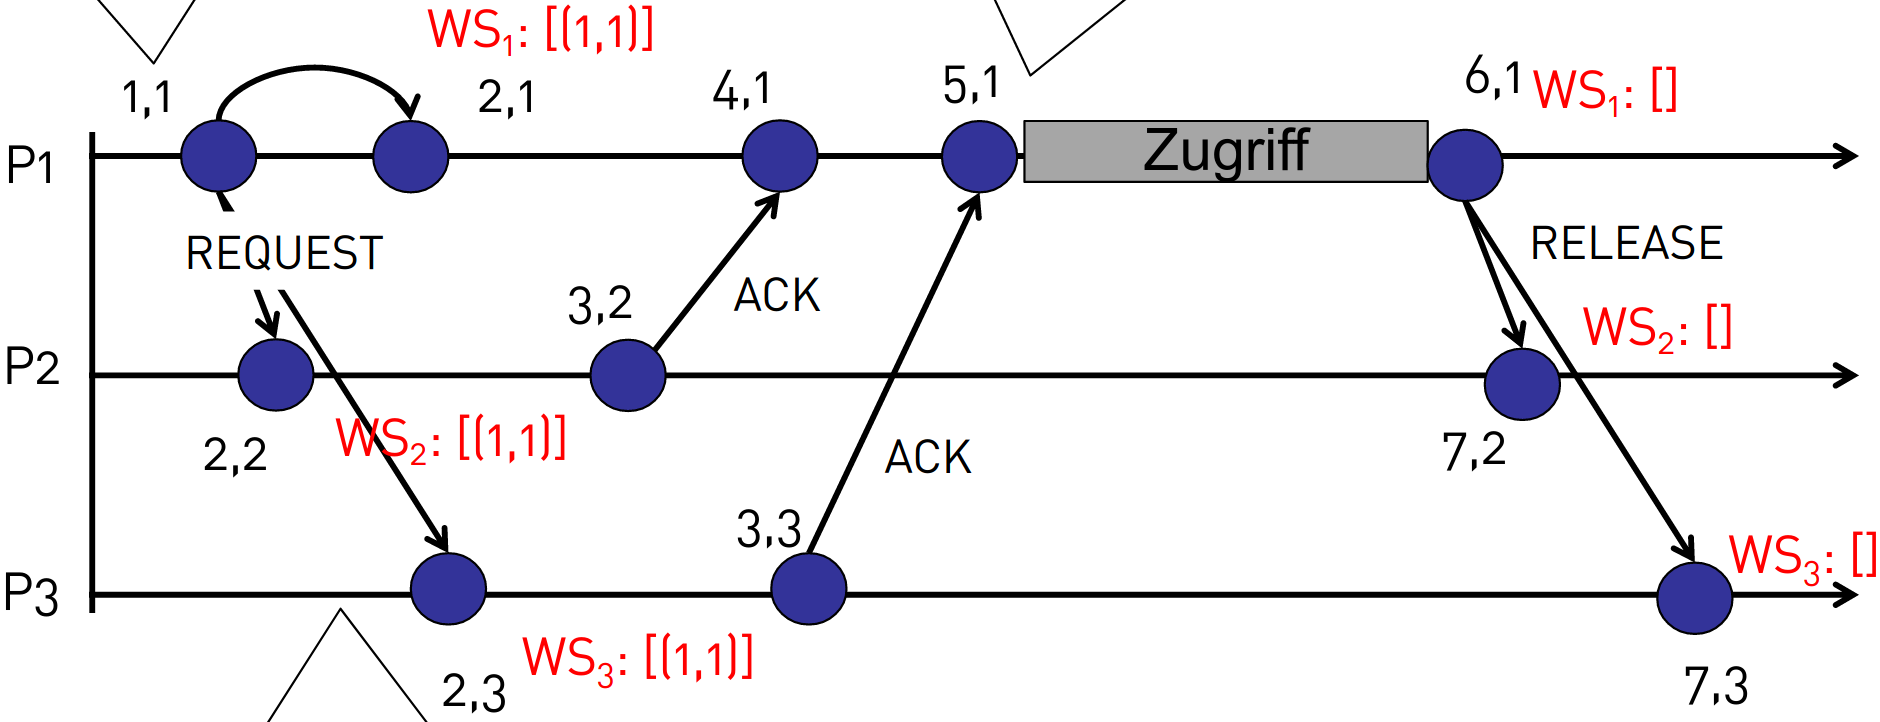
\includegraphics[height=150px]{Lamport-Algorithmus.png}

Beim Lamport-Algorithmus verwaltet jeder Prozess eine lokale Warteschlange mit REQUESTs. Das Vorgehen ist konkret wie folgt definiert:
\begin{enumerate}
    \item Wenn ein Prozess Zugriff auf die Ressource haben möchte, verschickt er ein REQUEST an alle anderen Prozesse
    \item Wenn ein Prozess eine REQUEST erhält, wird diese in die lokale, durch die Lamport-Time total geordnete Liste von REQUESTs eingefügt und \textbf{sofort} ein ACK zurückgesendet
    \item Wenn ein Prozess alle ACK zu seiner REQUEST bekommen hat und seine Request die kleinste Lamport-Time hat, kann er den Zugriff durchführen. Der Prozess kann sich sicher sein, dass es keine Requests mit einer niedrigeren Lamport-Time gibt, die er noch nicht erhalten hat, weil durch die Reihenfolgetreue der Nachrichten keine Nachricht mehr im Netzwerk sein kann, die vor den erhaltenen ACKs verschickt wurde
    \item Wenn ein Prozess seinen Zugriff beendet hat versendet er eine RELEASE Nachricht an alle anderen Prozesse, um die Ressource wieder freizugeben
    \item Wenn ein Prozess eine RELEASE-Nachricht empfängt, entfernt er den zugehörigen Eintrag seiner lokalen Warteschlange
\end{enumerate}

Der Algorithmus verlangt es, dass für jeden Zugriff auf die Ressource $3(n-1)$ Nachrichten versendet werden, wobei $n$ die Zahl der beteiligten Knoten im ist (jeweils ein REQUEST, ACK und RELEASE an alle anderen Knoten).

\subsubsection{Algorithmus von Ricart / Agrawala}

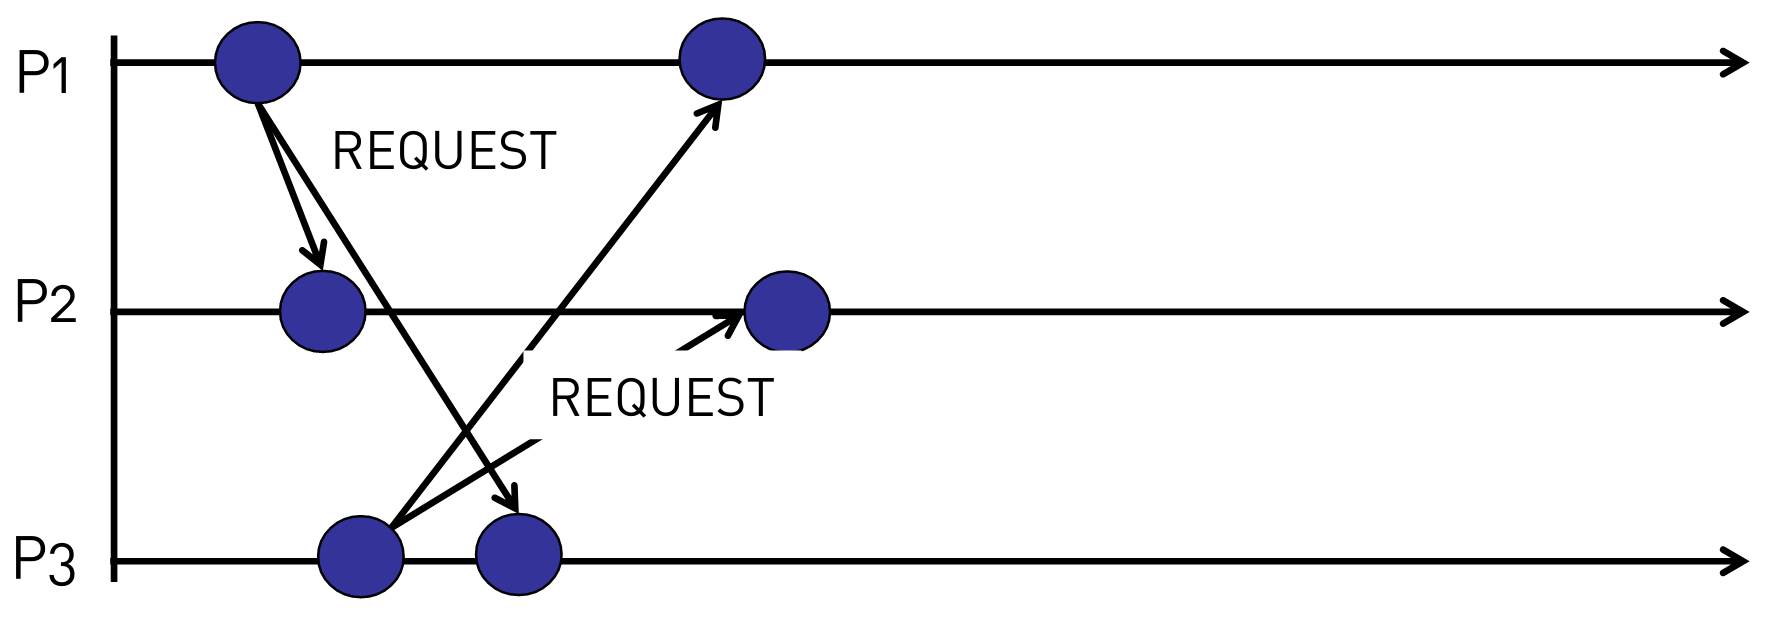
\includegraphics[height=130px]{Ricart-agragawa-algorithmus.png}

Der Algorithmus von Ricart und Argrawala verbessert den Lamport-Algorithmus hinsichtlich seiner Effizienz von $3(n-1)$ Nachrichten auf $2(n-1)$ Nachrichten pro Zugriff. Er modifiziert den Lamport-Algorithmus so, dass nur noch eine REPLY Nachricht anstatt der beiden Nachrichten ACK und RELEASE benötigt wird. Das Vorgehen ist wie folgt definiert:
\begin{enumerate}
    \item Wenn ein Prozess Zugriff auf die Ressource bekommen möchte sendet er ein REQUEST an alle anderen Prozesse (wie bei Lamport-Algorithmus)
    \item Wenn ein Prozess ein REQUEST erhält und selbst noch nicht auf REPLYs wartet (also zurzeit kein Interesse an Zugriff hat) oder die Lamport-Time der eingehenden REQUEST kleiner ist als die der eigenen REQUEST, sendet er sofort ein REPLY
    \item Wenn ein Prozess ein REQUEST erhält und selbst ein REQUEST mit einer kleineren Lamport-Time gesendet hat, sendet er das REPLY erst, wenn er seinen eigenen Zugriff auf die Ressource beendet hat
    \item Wenn ein Prozess alle REPLYs für seine Request erhalten hat, darf er auf die Ressource zugreifen
\end{enumerate}

Auf diese Weise werden erst immer alle REPLYs zu einem REQUEST erhalten, wenn es keine anderen REQUESTs mit einer niedrigeren Lamport-Time gibt. Auf diese Weise hat zu jeder Zeit nur max. 1 Prozess Zugriff auf die Ressource, nämlich der, der die REQUEST mit der niedrigen Lamport-Time gesendet hat.

\subsubsection{Eigenschaften der Algorithmen}

Für den Lamport-Algorithmus und den Algorithmus von Ricart / Agrawala gelten die folgenden Eigenschaften:
\begin{enumerate}
    \item \textbf{Deadlock-Freiheit}\\
          Da durch die totale Ordnung der Requests immer geregelt ist, wer Zugriff hat
    \item \textbf{Starvation-Freiheit}:\\
          Da das Empfangen einer ACK / RESPONSE Nachricht auf einem Knoten $K_{1}$ die eigene Lamport-Time erhöht, ist es für diesen Knoten erst möglich die nächste Response mit einer um $1$ höheren Lamport-Time als die anderen Knoten zu verschicken. Dadurch können auf jeden Fall andere Knoten auch zum Zuge kommen.
\end{enumerate}
\section{Konsistenz \& Konsistenzmodelle}

\subsection{Notation}

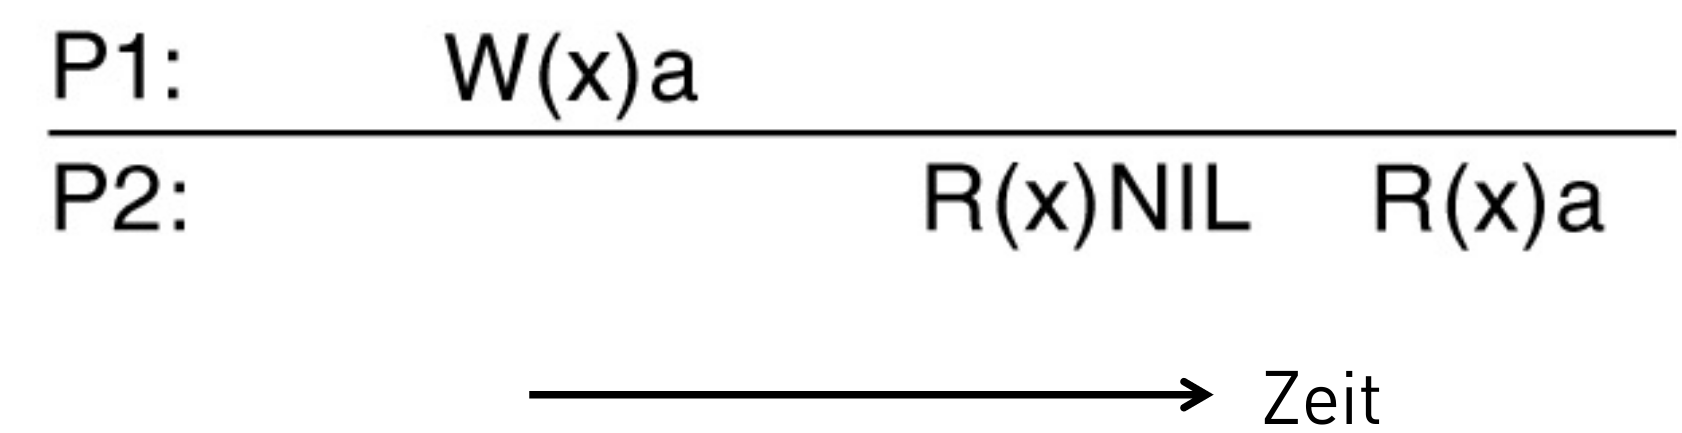
\includegraphics[height=60px]{NotationKonsistenz.png}

Im folgenden benutzen wir eine bestimmte Notation, um das Ergebnis von Schreibe- und Leseoperationen in einem verteilten System darzustellen. Wenn aus der Variable x der Wert a gelesen wurde oder in die Variable x der Wert a geschrieben wurde schreiben wir:\\

R(x)a \\
W(x)a \\

In dem oberen Diagramm bedeutet das, dass zuerst von P1 in die Variable x der Wert a geschrieben wird. Dann liest ein anderer Prozess P2 den Wert NIL (vgl. NULL) aus x. Offensichtlich ist das Ergebnis der Schreibeoperation von P1 noch nicht sichtbar. Dann liest P2 noch einmal den Wert von x und erhält nun den Wert a, d.h. offensichtlich wurde nun die Schreibeoperation mit P2 synchronisiert. Die Schreibeoperationen können jeweils auch als Nachricht betrachtet werden. Denn immer wenn auf replizierten Daten geschrieben wird bedeutet die Veröffentlichung dieses Schreibens, dass eine Nachricht an alle anderen Prozesse gesendet werden muss.

\subsection{Strikte Konsistenz}

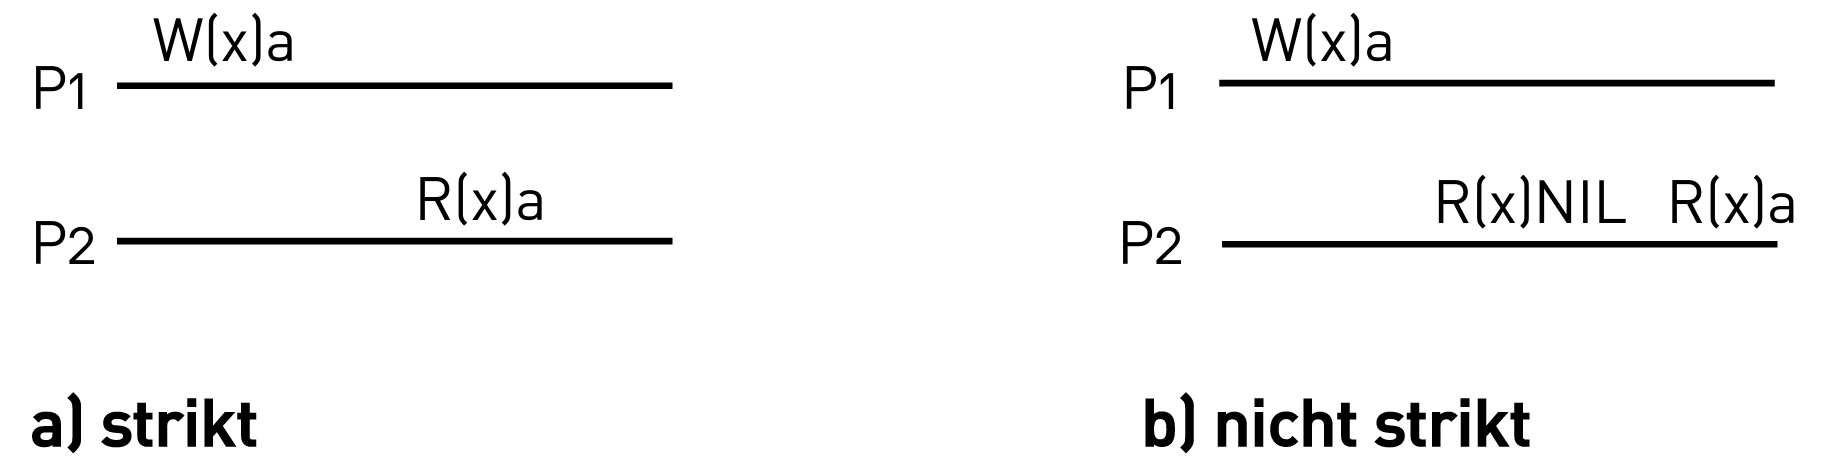
\includegraphics[height=85px]{strict-consistency.png}

Strikte Konsistenz bezeichnet, dass das Ergebnis jeder Leseoperation jeweils das Ergebnis der vorherigen Schreiboperation liefert. Strikte Konsistenz kann in einem Verteilten System nicht erreicht werden, weil die Veröffentlichung von Schreiboperationen Zeit benötigt in der das System zwangsweise inkonsistent ist.

\subsection{Sequentielle Konsistenz}

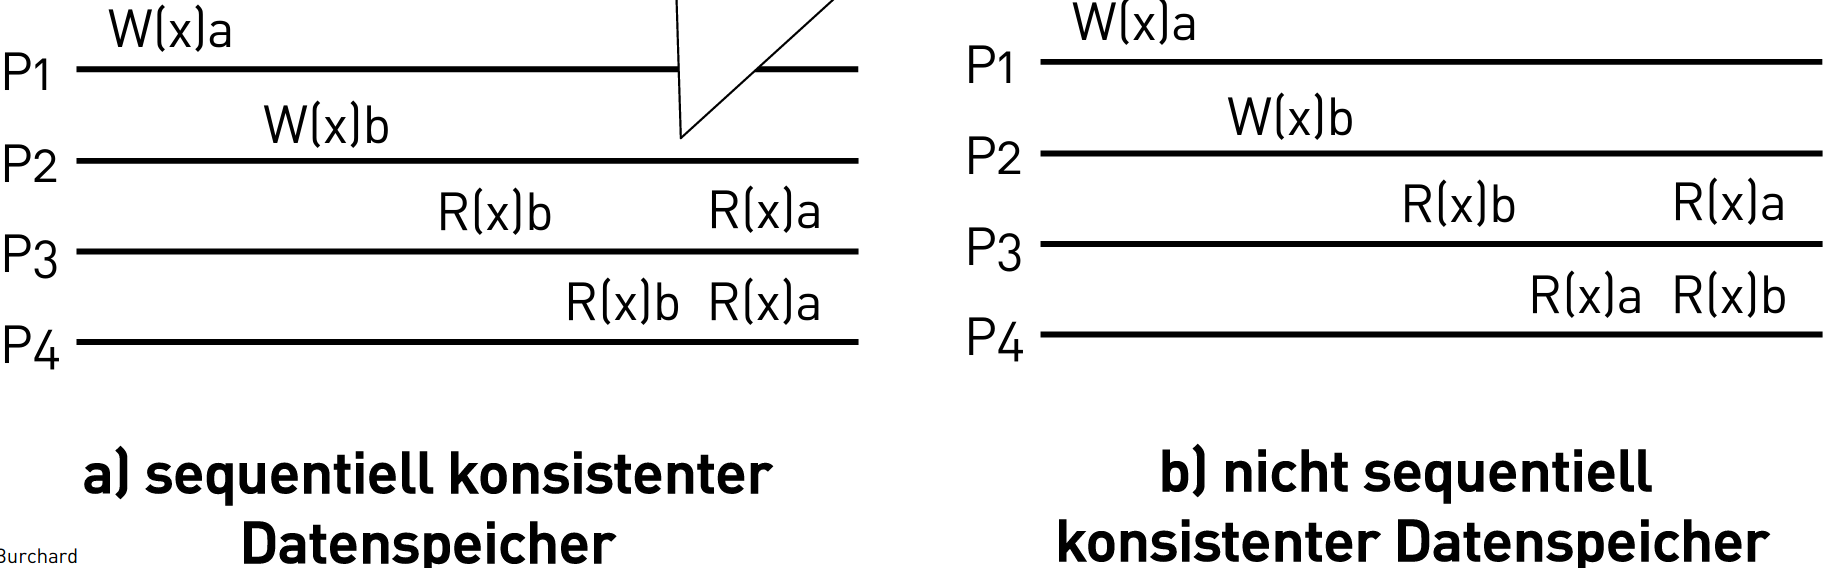
\includegraphics[height=100px]{sequential-consistency.png}

Sequentielle Konsistenz bedeutet, dass jeder Prozess bei seinen Leseoperationen die gleiche Reihenfolge von Veränderungen der Daten wahrnimmt. Nicht jeder Prozess muss jede Änderung lesen, aber wenn er sich dazu entscheidet zu lesen, dann muss die Reihenfolge der Änderungen, die gelesen werden würden, bei allen Prozessen gleich sein. \\
Dieses Konsistenzmodell lässt sich gut mit dem \hyperref[sec:master-slave]{Master-Slave-Cluster} implementieren, indem es einen Master gibt, der schreiben darf und viele Slaves, die lesen dürfen. Es gibt somit eine zentrale eindeutige Reihenfolge der Schreibeoperationen auf dem Master. Wenn zusätzlich gewährleistet wird, dass die Nachrichten, die der Master an die Slaves sendet, reihenfolgegetreu ankommen (z.B. mittels TCP), dann ist also auch gewährleistet, dass die Reihenfolge der Schreiboperationen, die auf den Slaves sichtbar ist, mit der Reihenfolge auf dem Master übereinstimmt.

\subsection{Kausale Konsistenz}

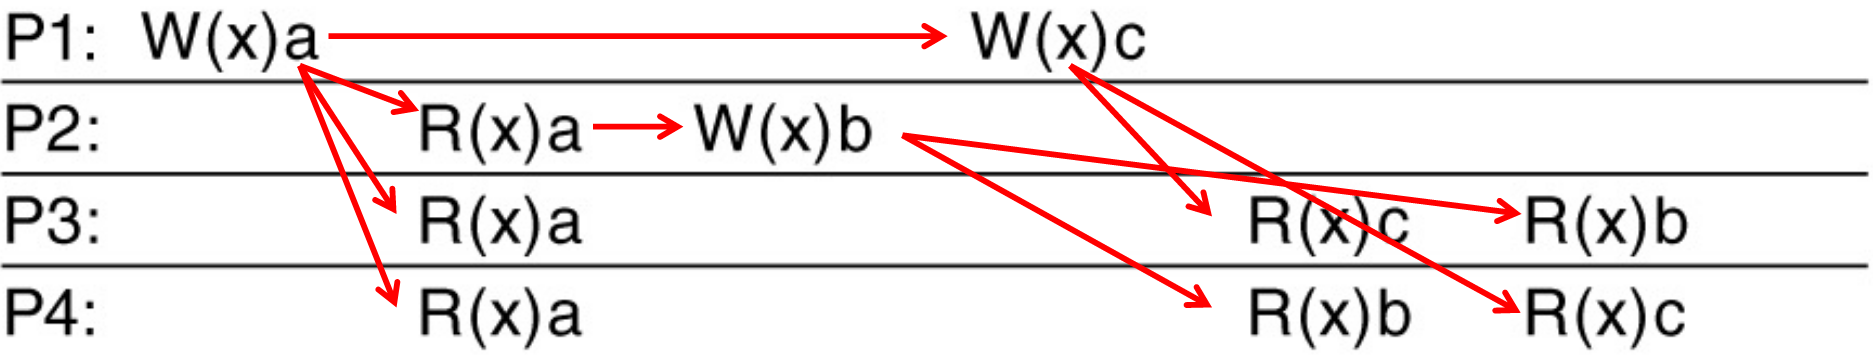
\includegraphics[height=70px]{causal-consistency-2.png}

Kausale Konstistenz ist gegeben, wenn sequentiell Konsistenz für alle Änderungen des Datenbestandes gegeben ist, die in kausalem Zusammenhang stehen könnten. Schreiboperationen $W_{1}(x)a$ und $W_{2}(y)b$ können dann in einem kausalen Zusammenhang stehen, wenn das Ergebnis von $W_{1}$ zur Zeit der Schreiboperation von $W_{2}$ bekannt ist, also wenn die Nachricht darüber, dass eine Schreiboperation stattgefunden hat, bereits erhalten wurde. Man kann sich vorstellen, dass die Schreiboperation $W_{2}$ (z.B. ein Like eines Beitrags in einem sozialen Netzwerk) nämlich nur durchgeführt worden sein könnte, weil bereits die Schreiboperation $W_{1}$ (z.B. die Veröffentlichung diese Beitrags) bekannt war. \\

In unseren Schaubildern soll ein roter Pfeil jeweils die Nachricht zeigen, welche die Änderung der Daten veröffentlicht. Jede Schreiboperation hat also $n-1$ Nachrichten zur Folge, wobei $n$ die Anzahl der Prozesse im verteilten System darstellt.\\
Im oberen Bild sehen wir also, dass ein kausaler Zusammenhang zwischen W(x)a und W(x)c, sowie zwischen W(x)a und W(x)b bestehen könnte. Es besteht allerdings kein kausaler Zusammenhang zwischen W(x)b und W(x)c. Das obere Schaubild bildet kausale Konsistenz ab, da $a \rightarrow b $ und $a \rightarrow c$ immer in dieser Reihenfolge gelesen werden. Die Reihenfolge, in der $b$ und $c$ gelesen werden, ist für die kausale Konsistenz nicht relevant und dürfte auch von verschiedenen Prozessen unterschiedlich wahrgenommen werden. \\

\subsubsection*{Implementierung kausaler Konsistenz mit Vektor-Time}

Um die kausale Konsistenz einzuhalten, muss ein Knoten beim Erhalt einer Nachricht (also einer Veröffentlichung einer Schreibeoperation) feststellen können, ob es eine Schreibeoperation gibt, von der die erhaltene Nachricht abhängen könnte, die er selbst noch nicht erhalten hat. \\
Um dies umzusetzen kann die  \hyperref[sec:vector-time]{Vektor-Time} der Nachrichten genutzt werden. Beim Erhalt einer Nachricht kann verglichen werden, ob irgendeine Komponente der Nachricht höher ist als die entsprechende Komponente der lokalen Vektor-Time. Dabei müssen aber nur die Komponenten anderer Prozesse, also nicht die des eigenen und nicht die des Senders der Nachricht, überprüft werden. Wenn dies der Fall ist, bedeutet das, dass der Absender zur Zeit des Sendens eine Nachricht von einem anderen Knoten erhalten haben muss, die der empfangene Knoten selbst noch nicht bekommen hat. Folglich ist es möglich, dass die Nachrichten in einem kausalen Zusammenhang stehen. Um kausale Konsistenz zu erreichen darf die Änderung an den eigenen Daten also erst sichbar werden, wenn die Nachricht(en), mit denen sie in kausalem Zusammenhang steht, auch eingetroffen sind. Falls also in der Zwischenzeit eine Schreiboperation (hier die in grau dargestellte) angefordert wird, so muss sie verzögert werden.

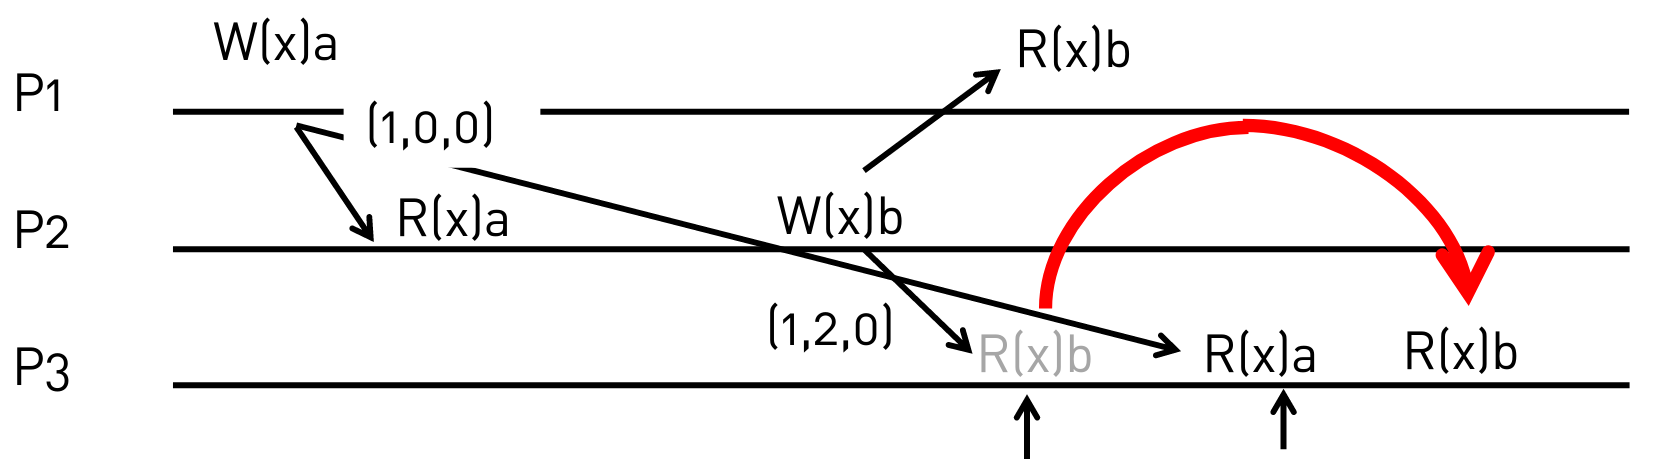
\includegraphics[height=90px]{causal-consistency-3.png}


\subsection{Urbildbasierte Protokolle}

Urbildbasierte Protokolle sind solche, die zu jeder Zeit nur genau einen Prozess des verteilten Systems schreiben lassen und dadurch sequentielle Konsistenz erreichen. Eine Implementierung ist das \hyperref[sec:master-slave]{Master-Slave-Cluster} mit einem Schreiber und vielen Lesern. Hierbei gibt es 2 grundlegende Weisen, wie man Schreibeoperationen umsetzen kann, die im Folgenden kurz beleuchtet werden sollen.

\subsubsection{Entferntes Schreiben}

Beim entfernten Schreiben werden Schreibeanfragen eines Slaves an den Server weitergeleitet, der diese dann durchführt.

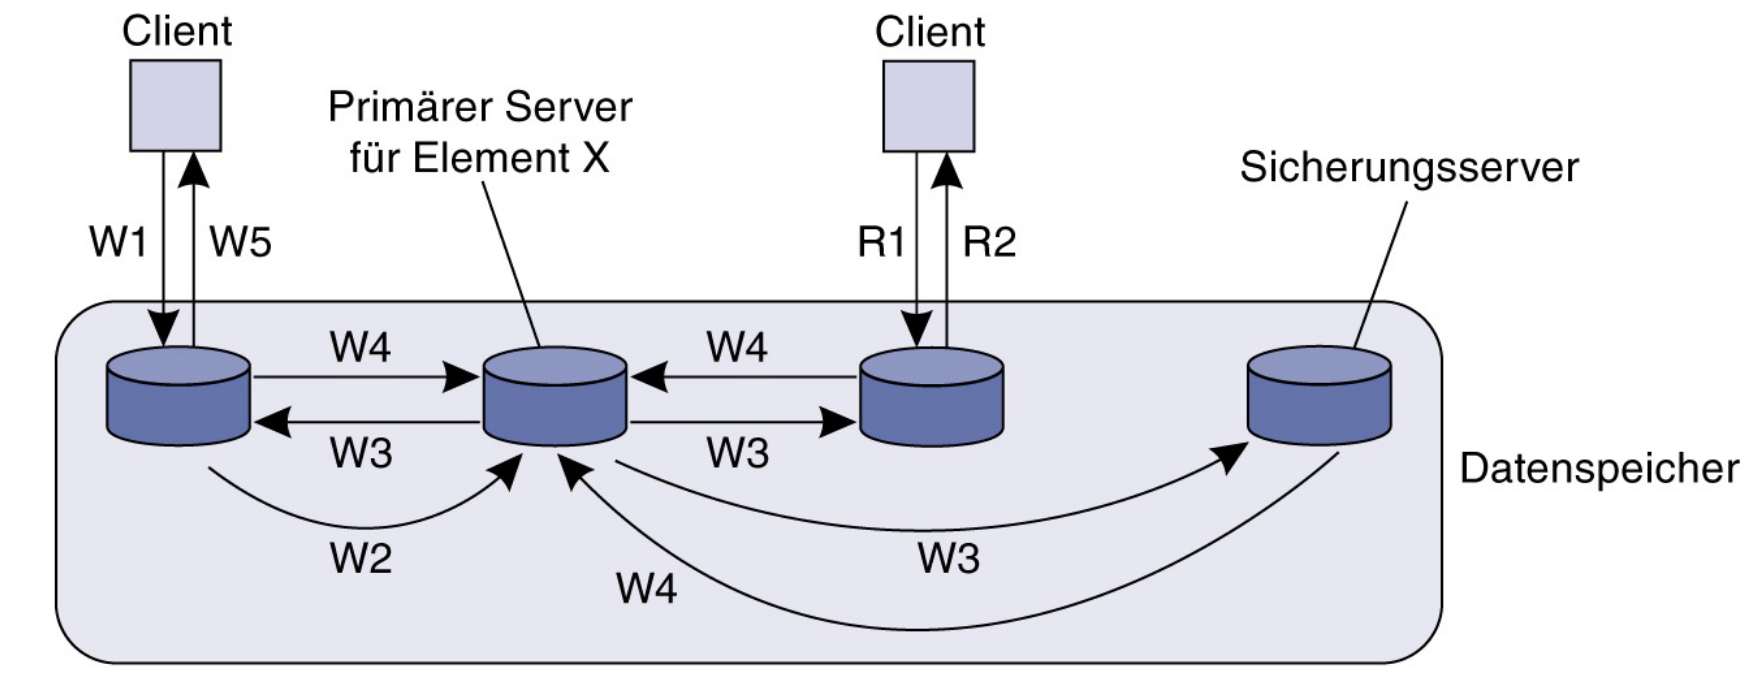
\includegraphics[height=150px]{entferntes-schreiben.png}

\subsubsection{Lokales Schreiben}

Beim lokalen Schreiben wird zunächst die benötigte Ressource vom Master auf einen Slave kopiert, sodass dieser den aktuellsten Stand dieser Ressource hat. Dann wird dieser Slave zum Master ernannt und die Schreiboperation kann direkt lokal ausgeführt werden. Diese Variante erfordert mehr Logik und Aufwand für das Kopieren. Allerdings kann sie performanter sein, wenn ein Client in der Regel sehr viele Daten schreibt. In diesem Fall werden nämlich viele Nachrichten über das Netzwerk vermieden.

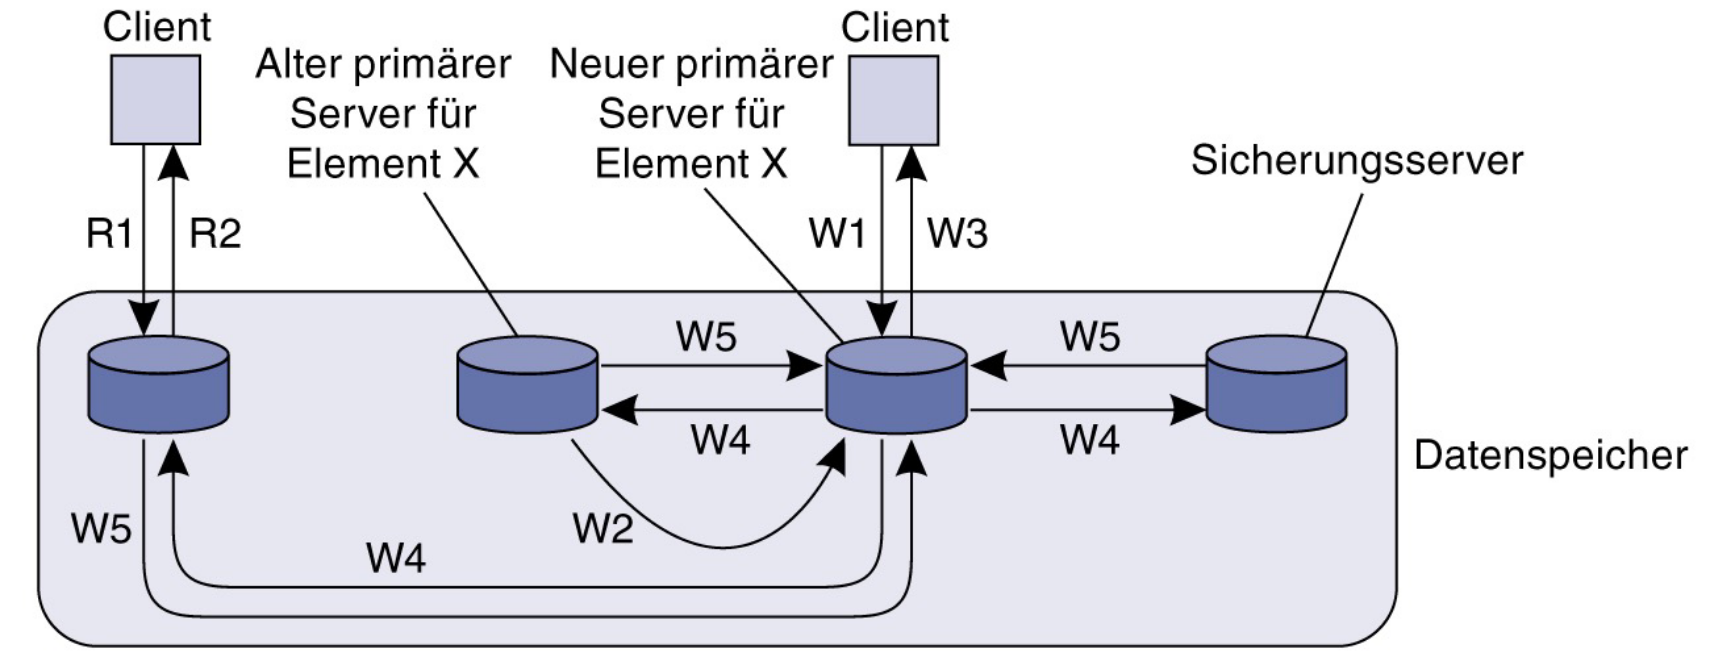
\includegraphics[height=150px]{lokalesSchreiben.png}


\subsection{Transaktionsbasierte Protokolle}

\subsection{Prinzip von Transaktionen}

Transaktionen werden so aufgefasst, dass für eine Menge von schreibenden Operationen, die als Transaktion zusammengefasst werden, die ACID Prinzipien gelten, wie man sie von Datenbanken kennt:
\begin{itemize}
      \item \textbf{A}tomicity
      \item \textbf{C}onsistency
      \item \textbf{I}solation
      \item \textbf{D}urability
\end{itemize}

In einem verteilten System wird die Schwierigkeit erhöht, da verlangt wird, dass auf einer bestimmten Menge von Remote-Rechnern eine Transaktion durchgeführt werden soll.

\subsubsection{2-Phasen-Commit}
\label{sec:2pc}
Der 2-Phasen-Commit, kurz 2PC, ist ein Protokoll, dass gewährleisten soll, dass eine Transaktion auf allen oder auf keinem Rechner aus einer Menge von Remote-Rechnern durchgeführt wird. Führt also ein Rechner lokal ein ABORT aus, so sollen andere Rechner auch einen ABORT ausführen, der ABORT soll also global gelten. Ein globaler COMMIT gelingt genau dann, wenn er bei jedem Rechner lokal gelingt.\\

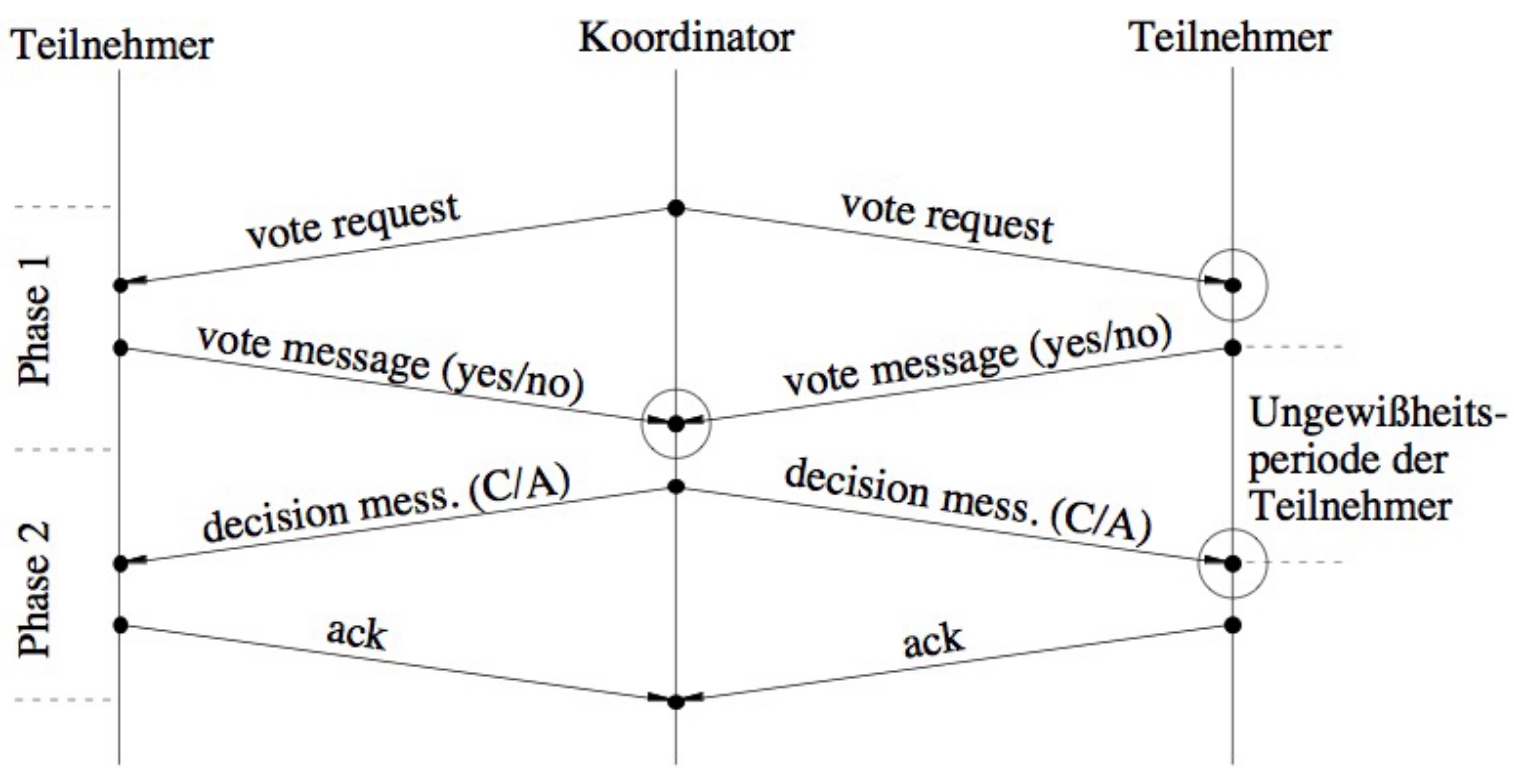
\includegraphics[height=200px]{2pc-nachrichtenfluss.png}

In 2PC haben wir einen lokalen Koordinator und $n$ Teilnehmer. Der Koordinator macht die globalen Entscheidungen über ABORT und COMMIT und kommuniziert sie mit allen Teilnehmern. Das System ist also im Sinne eines Master-Slave-Clusters aufgebaut, dass den Koordinator als schreibende Einheit hat. In dem Beispielbild gehen wir davon aus, dass die Transaktion bereits vom Koordinator begonnen wurde und er auch schon fertig mit Schreiben ist, da der eigentlich spannende Teil natürlich der COMMIT ist.\\
Damit der Koordinator eine Entscheidung treffen kann, sodass die oben gestellten Forderungen gelten, muss er, bevor er einen globalen COMMIT verkündet, sicher sein, dass alle Rechner diesen COMMIT auch durchführen können. Deshalb sendet er zunächst einen Vote-request an alle Teilnehmer. Die Teilnehmer antworten darauf mit der Information, ob sie den COMMIT in der Zukunft auf jeden Fall durchführen können oder nicht. Wenn die Antwort von allen Knoten eingetroffen ist kann der Koordinator die Entscheidung treffen, die er allen Teilnehmern sendet. Diese Führen dann die Operation, also COMMIT oder ABORT lokal aus.\\
Man kann das Verfahren auch als State-Machine visualisieren:

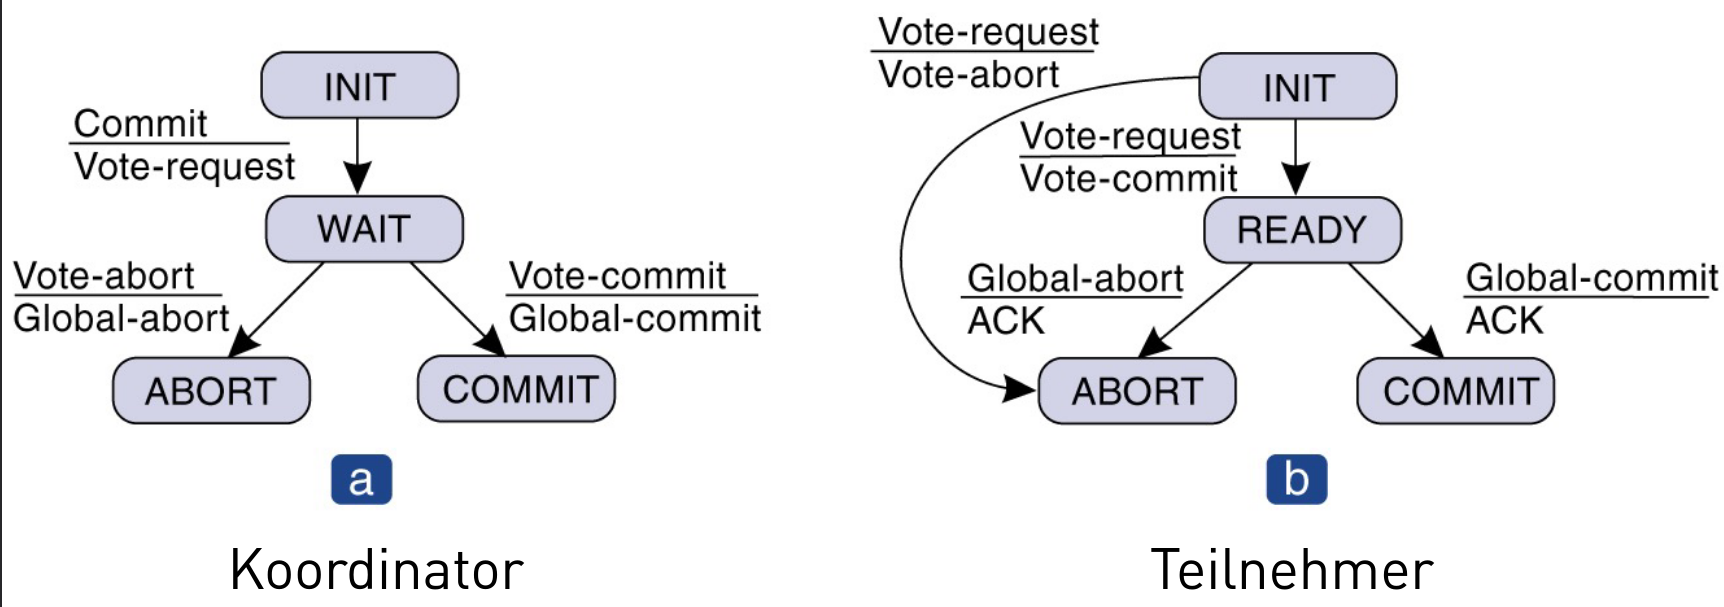
\includegraphics[height=150px]{2pc-state-machine.png}

Das 2PC-Protokoll hat aber Probleme bezüglich Fehlertoleranz. In der Zeit in der ein Teilnehmer schon mit einer Vote Message abgestimmt hat, aber noch keine Antwort über das Ergebnis vom Koordinator erhalten hat, ist er nicht handlungsfähig. Er darf weder die Transaktion ABORTen, da er schon zugesagt hat, dass er sie in der Zukunft COMMITen könnte, noch darf er sie COMMITen, da er noch kein grünes Licht vom Koordinator bekommen hat. Damit ein Teilnehmer nicht ewig in solch einem Zustand verweilt, ist es sinnvoll einen Timout zu setzen. Die Frage ist nur, was der Teilnehmer machen soll, wenn es zu einem Timeout kommt. Die Antwort auf diese Frage liefert das Terminierungsprotokoll.\\
Laut dem \textbf{Terminierungsprotokoll} soll ein Teilnehmer bei einem Timeout einen anderen Knoten q um Hilfe fragen. Es gibt 3 Möglichkeiten wie q antworten kann:
\begin{enumerate}
      \item q hat die Entscheidung des Koordinators bereits erhalten und gibt sie an den Fragenden weiter
      \item q hat selbst noch kein Vote abgegeben und kann daher für ABORT voten, um dafür zu sorgen, dass die globale Entscheidung ein ABORT wird
      \item q befindet sich auch im wartenden Zustand und kann nicht helfen
\end{enumerate}

Kritisch ist der dritte Fall, für den es tatsächlich keine Lösung gibt.\\

Außerdem sollten wir uns über \textbf{Crash Recovery} Gedanken machen, also über die Frage was ein Rechner tun soll, wenn er nach einem Ausfall wieder online ist. Die Lösung ist jeden Zustandsübergang auf die Festplatte zu schreiben, sodass bei der Recovery die Information von dort genutzt werden kann, um fortzufahren.\\

Obwohl das 2PC-Protokoll scheitert, wenn alle Rechner in einem wartenden Zustand sind, also das Terminierungsprotokoll nicht erfolgreich ist, ist es dennoch praktisch einsetzbar, falls genau solch ein Zustand anderweitig verhindert werden kann. Zum Beispiel in Datacentern, in denen es selten vorkommt, dass Rechner nicht erreichbar sind, ist eine Vermeidung dieses Fehlerzustands mit statistisch hoher Wahrscheinlichkeit gegeben.

\subsubsection{Quoren}
\label{sec:quorums}

Die Idee von Quoren ist, dass wir nicht gewährleisten müssen, dass alle Rechner des Clusters eine Transaktion committen. Stattdessen können wir verlangen, dass bloß mindestens eine Teilmenge der Rechner die Transaktion committen und wir beim Lesen sicherstellen, dass wir die Information von einem dieser Rechner erhalten.\\

Um das zu gewährleisten definieren wir folgende Quoren (minimale Anzahl für die Durchführung einer Operation) bei $n$ Teilnehmern:
\begin{enumerate}
      \item Schreibquorum QW $> \frac{n}{2}$
      \item Lesequorum QR mit $QR + QW > n$
\end{enumerate}

Um eine Operation global durchzuführen, muss sie also auf mindestens so vielen Teilnehmern des Rechnernetzes durchgeführt werden, wie wir im Quorum festgelegt haben. Mit der ersten Bedingung stellen wir sicher, dass es nicht mehrere parallele Schreiboperationen geben darf. Mit der zweiten Bedingung stellen wir sicher, dass beim Lesen von Daten für jeden Datensatz mindestens einer der antwortenden Rechner die aktuellste Version zu diesem Datensatz zurückliefert. Das liegt daran, dass durch die beiden Quoren gewährleistet ist, dass die Menge der lesenden Rechner und die Menge der schreibenden Rechner für jede Transaktion nicht disjunkt sind. Nun muss man nur noch herausfinden, welches der gelesenen Replikate das aktuellste ist. Das kann mithilfe von \hyperref[sec:logic-time]{logischer Zeit} erreicht werden.\\

Bei der Benutzung von Quoren muss es nicht zwangsläufig einen Koordinator geben, d.h. das System kann so designed werden, dass jeder Knoten schreiben darf. In diesem Fall kann es zu Deadlocks kommen, wenn ein Rechner, der eine Schreibanfrage stellt und schon einige Rechner für das Schreiben allokiert hat, so lange wartet, bis er genug Rechner allokieren kann und das Quorum erreicht ist und gleiches parallel von einem anderen Rechner getan wird. Allerdings kann dies leicht mit Timeouts gelöst werden, bei deren Auftritt nach einem zufälligen Zeitintervall ein erneuter Versuch gestartet wird.\\

Abschließend lässt sich sagen, dass Quoren den Aufwand beim Schreiben verringern, aber den Aufwand beim Lesen vergrößern, da nun nicht mehr nur von einem einzigen Rechner, sondern von mehreren gelesen werden muss.

\subsubsection{Fehlerbehandlung}

Es gibt verschiedene Arten, wie wir in einem verteilten System mit dem versenden von Nachrichten, bzw. mit Schreibeoperationen umgehen können, die wir Fehlersemantiken nennen:

\begin{enumerate}
      \item \textbf{Maybe:}\\
            Eine Nachricht wird genau einmal versendet und es gibt keine Fehlerbehandlung
      \item \textbf{At-most-once:}\\
            Falls ein Fehler auftritt versenden wir die Nachricht erneut. Allerdings stellen wir sicher, dass das Duplikate der Nachricht auf dem Server erkannt werden, sodass die Nachricht effektiv nur einmal eintritt. \textit{At-least} bedeutet, dass es vorkommen kann, dass auch bei mehrmaligem erneuten Versuchen der Server nicht erreicht werden kann.
      \item \textbf{At-least-once:}\\
            Eine Nachricht wird so oft gesendet, bis sie ankommt. Es werden keine Duplikate herausgefiltert. Daher ist diese Methode nur für idempodente Operationen sinnvoll.
      \item \textbf{Exactly-once:}\\
            Es wird sichergestellt, das die Anfrage genau einmal vom Server bearbeitet wird. In der Praxis ist es nicht möglich das vollständig zu ermöglichen. Es sollte daher geklärt werden, was in einer konkreten Implementierung dieser Fehlersemantik gewährleistet wird. In der Regel läuft es darauf hinaus, dass diese Fehlersemantik eigentlich hätte \textit{at-most-once} genannt werden sollen.
\end{enumerate}

Wir wollen uns nun überlegen, was sinnvoll wäre, um eine \textbf{at-most-once} Fehlersemantik zu implementieren. Die Fehlersituation, die wir dazu im Folgenden betrachten wollen ist folgende:
\begin{enumerate}
      \item Ein Client hat eine Anfrage für eine Schreiboperation an einen Server gesendet. Dann hat er nach einiger Zeit keine Reaktion vom Server erhalten und reagiert mit einem Timeout.
      \item Der Client sendet die Anfrage erneut
      \item Durch eine eindeutige ID ist gekennzeichnet, dass die beiden Nachrichten des Clients zur selben Operation gehören
\end{enumerate}

Diese Situation kann verschiedene Ursachen haben, bei denen es verschiedene Dinge zu beachten gilt:
\begin{itemize}
      \item Die Request-Nachricht des Clients ging im Netzwerk verloren:\\
            In diesem Fall kann genau die selbe Nachricht nocheinmal gesendet werden, da dieser Zustand äquivalent zum Zustand vor dem ersten Senden der Nachricht ist.
      \item Serverabsturz:\\
            Verhält sich wie 1.
      \item Die Response-Nachricht des Servers (z.B. ein ACK) ging im Netzwerk verloren:\\
            In diesem Fall muss der Server erkennen, dass die Nachricht bereits verarbeitet wurde und sollte die angefragte Operation nicht erneut durchführen. Die Antwort ist möglicherweise noch gecached und kann demnach von dort direkt entnommen werden.
      \item Der Server ist zwar online, aber so langsam, dass das Timout entsteht:\\
            In diesem Fall ist eine Prävention des Timeouts sinnvoll, indem der Server eine vorläufige Antwort schickt, die suggeriert, dass die tatsächliche Antwort mit Verzögerung gesendet werden wird.
\end{itemize}
\section{Verteilte Dateisysteme}

\subsection{Was ist ein verteiltes Dateisystem?}

Ein verteiltes Dateisystem ist ein Dateisystem, das die Speicherung von Daten auf mehrere Rechner verteilt. Dabei kann sowohl die Segmentierung von Daten, d.h. die Daten werden in verschiedene Bereiche unterteilt, wobei jeder Rechner einem anderen Bereich zugeordnet ist, als auch Replikation, d.h. mehrere Rechner speichern die selben Daten, um Ausfallsicherheit und andere Ziele von VS zu erreichen, vorliegen.

\subsubsection{Zugriffsmodelle}
\label{sec:zugriffsmodelle}
Wir unterscheiden zwischen den folgenden beiden Zugriffsmodellen verteilter Dateisysteme:
\begin{itemize}
    \item \textbf{Remote Access:}\\
          Hierbei finden alle schreibenden Zugriffe auf dem Server statt. Dazu ist eine komplexe Schnittstelle zwischen Client und Server nötig. Es entsteht eine dauerhafte Nutzung des Netzwerks mit kleinen Datenmengen
    \item \textbf{Upload/Download:}\\.
          Der Client kopiert zu Beginn eine Datei vom Server in seinen lokalen Speicher. Dann nimmt er dort Schreiboperationen vor und kopiert die Datei zurück auf den Server, wo sie dann gemerged wird. Die Schnittstelle, die benötigt wird ist also simpler. Das Netzwerk wird nur beim Öffnen und Schließen (impliziert download und upload) benötigt, dabei werden aber möglicherweise große Datenmengen übertragen.
\end{itemize}

\subsubsection{Schnittstellen-Design}
Eine wesentliche Eigenschaft der Schnittstelle eines verteilten Dateisystems ist, ob es zustandslos oder zustandsbehaftet ist.
\begin{itemize}
    \item \textbf{Zustandslos:}\\
          \begin{itemize}
              \item Im Server wird kein Speicher für den Status der Client-Verbindungen benötigt. Alle Informationen werden stattdessen in jedem Aufruf (jeder Nachricht) übertragen.
              \item Es gibt keine Operationen zum Öffnen oder Schließen von Dateien.
              \item Fehlertoleranter und einfacher zu implementieren, da nicht mit Verbindungsabbrüchen umgegangen werden muss.
          \end{itemize}
    \item \textbf{Zustandsbehaftet:}\\
          \begin{itemize}
              \item Nachrichten werden kürzer, da gewisse Informationen schon implizit im Verbindungsstatus vorliegen.
              \item Precaching möglich, da in Mitten einer Session schon bekannt ist, auf welche Datei ein Client zugreifen möchte.
              \item Locks (Sperren) sind einfach zu realisieren.
          \end{itemize}
\end{itemize}

\subsection{Network File System - NFS v4}

Das Network File System ist ein Netzwerkprotokoll, das implementiert werden kann, um ein verteiltes Dateisystem zu implementieren. Der Zugriff auf Dateien erfolgt für den Benutzer genau so, als ob die Dateien lokal gespeichert wären. NFS hat folgende Eigenschaften
\begin{itemize}
    \item NFS v4 ist \textbf{zustandsbehaftet}. Eine Datei wird mit verschiedenen Aufrufen geöffnet, gelesen geschrieben, geschlossen usw.. Die Vorgängerversion NFS v3 war allerdings zustandslos.
    \item Die \hyperref[sec:zugriffsmodelle]{Zugriffsart} ist \textbf{Remote-Access}.
    \item Die Änderungssemantik ist \textbf{Sitzungssemantik}. Das heißt, dass Änderungen an Dateien beim schließen der Datei sichtbar werden.
\end{itemize}

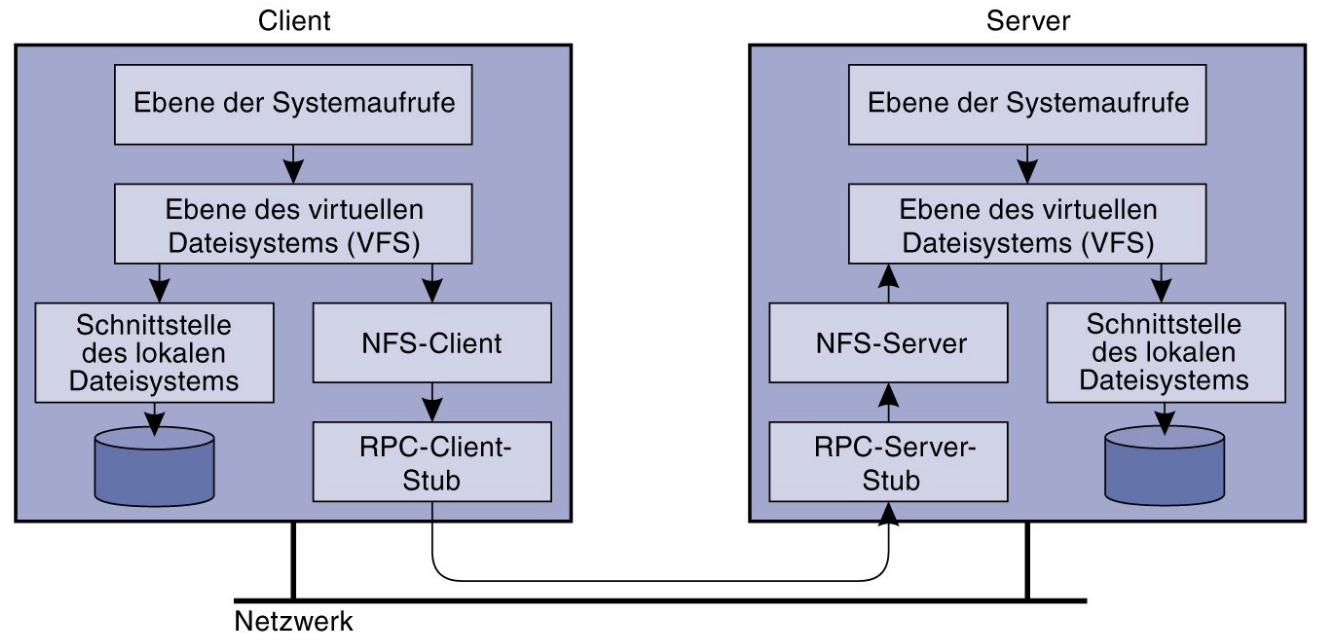
\includegraphics[height=150px]{nfs-architecture.png}


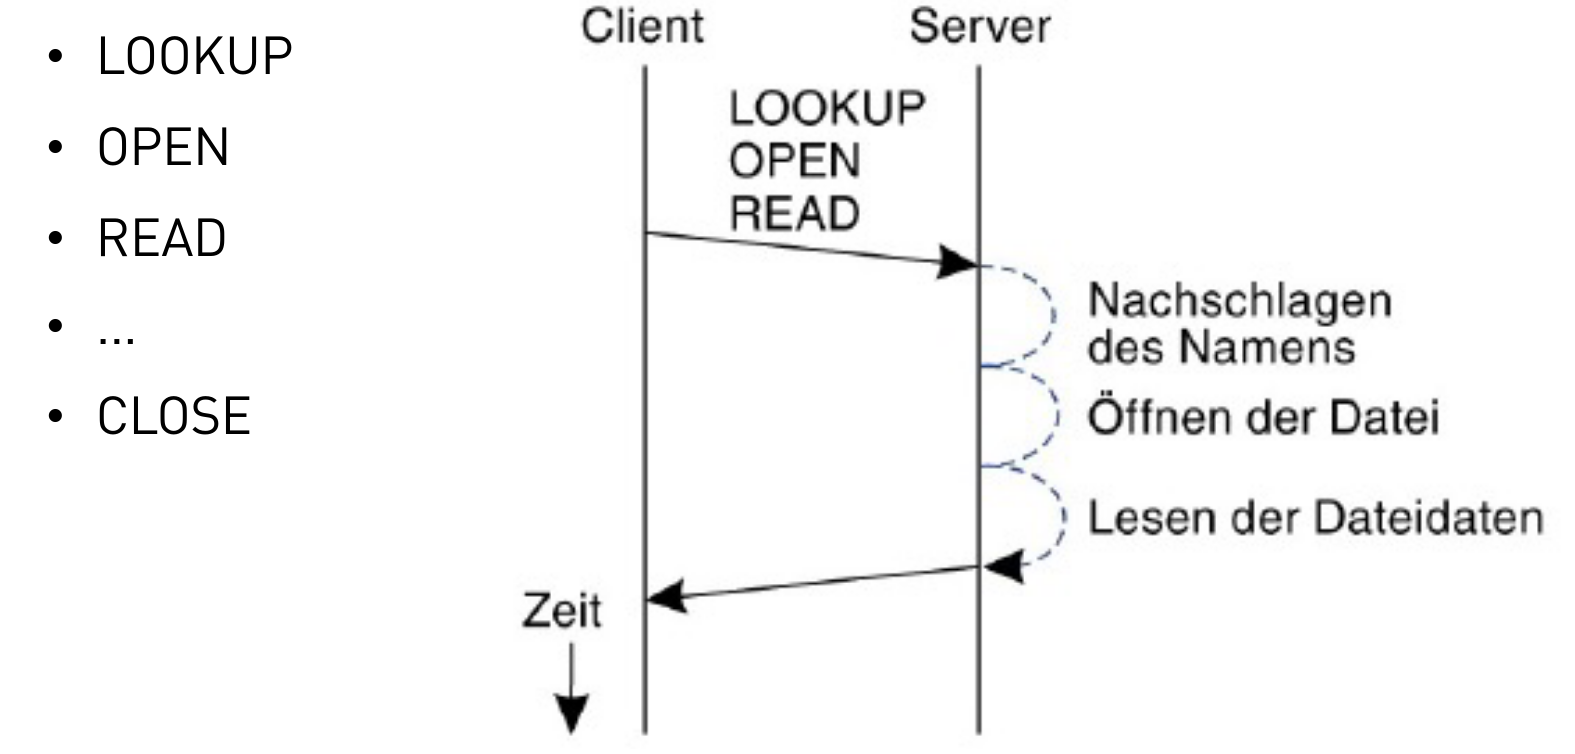
\includegraphics[height=150px]{nfs-sequence.png}

NFS basiert auf RPC. NFS v4 erlaubt es in einem RPC-Call mehrere Funktionsaufrufe zu übertragen. Im oberen Beispiel sehen wir z.B. wie ein LOOKUP, ein OPEN und ein READ zusammen übertragen werden, ausgeführt werden und dann nur das Gesamtergebnis zurückgeliefert wird.
\begin{itemize}
    \item \textbf{LOOKUP} liefert zunächst alle Server auf denen eine bestimmte Datei existiert.
    \item \textbf{READ} übernimmt eine Startposition und eine Anzahl an Bytes. Der Server wird dann diese Daten zurückliefern. Allerdings kann der Server auch weniger Daten zurückliefern, falls er der Meinung ist, dass die angefragte Datenmenge zu groß für einen einzigen RPC-Call ist.
\end{itemize}

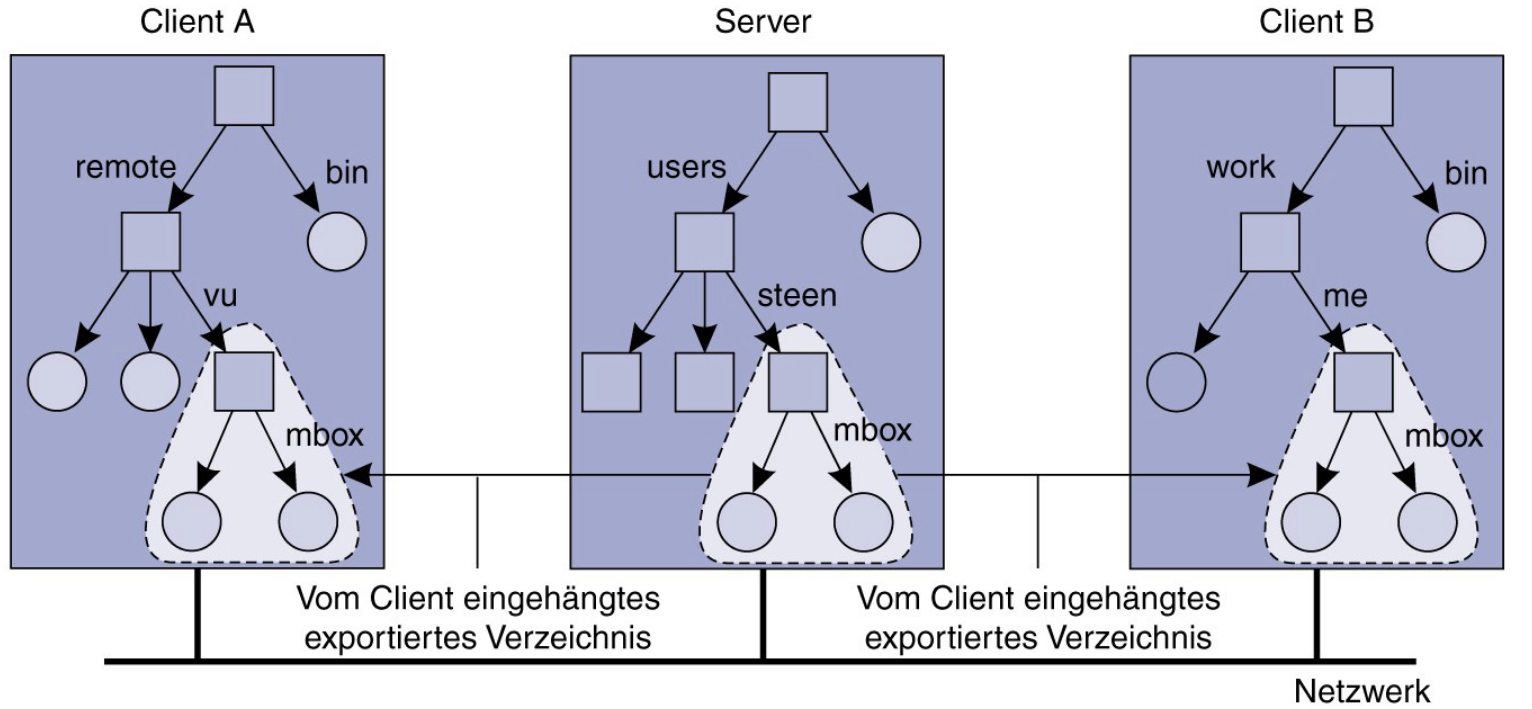
\includegraphics[height=150px]{nfs-mounting.png}

Um das verteilte Dateisystem in das eigene lokale Dateisystem einzubinden, kann es in den lokalen Verzeichnisbaum gemountet werden.

\subsubsection*{Locks}

NFS v4 ermöglicht es auch Sperren zu setzen. Man kann sowohl Schreib- als auch Lesesperren setzen. Durch diese Maßnahmen kann die Konsistenz des Systems durch den Benutzer bei kritischen Operationen sichergestellt werden.

\subsection{Google File System - GFS}
\label{sec:gfs}

Das Google File System ist ein von Google entwickeltes verteiltes Dateisystem, das auf Linux-Rechnern einsetzbar ist. Es ist auf große Datenmengen mit großen Dateien (über 100GB) optimiert. Der Haupteinsatzzweck ist die Verwendung im Zusammenhang mit Map-Reduce Operationen auf Basis von Suchanfragen. Bei der Entwicklung des Systems wurden folgende Annahmen gemacht:
\begin{itemize}
    \item Die Dateien sind enorm groß.
    \item Es gibt enorm viele Dateien.
    \item Das System wird von handelsüblichen Rechnern gehosted, die häufig ausfallen können.
    \item Dateien werden entweder gelesen oder es werden Daten angehängt. Das Ändern oder Löschen von bestehenden Daten kommt äußerst selten vor.
    \item Bandbreite ist wichtiger als Latenz, da große Datenmengen übertragen werden.
\end{itemize}

\subsubsection*{Systemdesign}

Dateien werden in mehrere 64MB große Chunks unterteilt. Jeder Chunk kann durch eine eindeutige ID, das chunk handle, identifiziert werden. Diese Chunks können dann auf mehrere Rechner aufgeteilt werden, sodass eine Datei nicht komplett auf einem einzigen Server liegen muss. Im GFS gibt es 2 Komponenten:
\begin{itemize}
    \item Einen \textbf{Master-Server:}\\
          Der Master Server speichert Metainformationen über den Zustand des Systems. Er weiß, welche Dateien es gibt, welche Chunks auf welchen Servern liegen und wie groß die Dateien sind. Diese Information bekommt er über zyklisches Abfragen aller Chunk-Server, die sogenannten Heart-Beat-Messages. Alle Anfragen von Clients, sowohl lesende als auch schreibende, laufen über diesen Master. Er liefert dem Client dann das chunk handle und die Adresse des zuständigen Chunk-Servers. Dann kann der Client seine Anfrage direkt an den Chunk-Server stellen. Damit der Master-Server nicht zum Bottleneck oder zur Schwachstelle werden kann, gibt es sogenannte Shadow-Master. Die Shadow-Master übernehmen zusätzlich die Koordination von Leseanfragen und springen für den richtigen Master-Server ein (siehe \hyperref[sec:fail-over-cluster]{Fail-Over-Cluster}).
    \item Sehr viele \textbf{Chunk-Server:}\\
          Die Chunk Server speichern einen ihnen zugewiesenen Teil der Chunks lokal in einem Linux-Dateisystem. Um Ausfallsicherheit zu gewährleisten, werden die Daten repliziert, sodass jeder Chunk auf mindestens 3 Chunk-Servern gespeichert ist. Jedem Chunk wird vom Master-Server ein bestimmter Chunk-Server als primary replica zugeordnet. Schreiboperationen werden dann zuerst auf dem primary replica ausgeführt und von dort aus mit einem \hyperref[sec:2pc]{2-Phasen-Commit} mit den anderen Chunk-Servern synchronisiert. Leseoperationen können auf jedem beliebigen Chunk durchgeführt werden, da diese Chunks durch die Synchronisierung mittels 2PC alle konsistent sein sollten. Das verfahren ist also ein \hyperref[sec:quorums]{Quorum} mit QW=n und QR=1. Hierbei entspricht n aber der Anzahl der Server auf denen das Chunk repliziert ist, also mindestens 3, und nicht der Anzahl der Gesamtrechner.
\end{itemize}

GFS verfolgt also eine \hyperref[sec:master-slave]{Master-Slave-Architektur}

\subsection{Andrew File System - AFS}

Das AFS ist ein verteiltes Dateisystem, das für die Carnegie Mellon University mit dem Fokus auf Skalierbarkeit entwickelt wurde. Es basiert auf RPC und wird auch im WAN genutzt.

\subsection{Hadoop Distributed File System - HDFS}

Das Hadoop Distributed File System ist ein verteiltes Dateisystem, das Teil von Apache Hadoop ist und daher speziell für \hyperref[sec:map-reduce]{Map-Reduce} optimiert ist. Es ist ähnlich aufgebaut wie das \hyperref[sec:gfs]{GFS}.

\end{document}
